% Necoyoad Architecture Blueprint v2 — Source-Verified
% Builds on v1 (SQL-only) by reading the actual PHP source (1,450 files).

\documentclass[11pt,a4paper]{article}

% ============================================================
%  Packages
% ============================================================
\usepackage[T1]{fontenc}
\usepackage[utf8]{inputenc}
\usepackage{lmodern}
\usepackage{microtype}

\usepackage{graphicx}
\usepackage{xcolor}
\usepackage{geometry}
\usepackage{amsmath}
\usepackage{amssymb}

\usepackage{tcolorbox}
\tcbuselibrary{skins,breakable,listings}
\usepackage{colortbl}
\usepackage{booktabs}
\usepackage{tabularx}
\usepackage{longtable}
\usepackage{array}
\usepackage{enumitem}
\usepackage{adjustbox}
\usepackage{caption}
\usepackage{fancyhdr}
\usepackage{titlesec}
\usepackage{pdflscape}
\usepackage{listings}

% TikZ
\usepackage{tikz}
\usetikzlibrary{arrows.meta,positioning,calc,shapes.geometric,fit,backgrounds,chains,decorations.pathreplacing,shapes.multipart}

% hyperref - last
\usepackage[
    colorlinks=true,
    linkcolor=blue!50!black,
    citecolor=blue!40!black,
    urlcolor=blue!60!black,
    bookmarks=true,
    bookmarksnumbered=true,
    unicode=true,
    pdftitle={Necoyoad - Source-Verified Architecture Blueprint (v2)},
    pdfauthor={Reverse-Engineered Architecture Report},
    pdfsubject={Software Architecture, PHP Source Analysis, OpenCart-derived CMS},
    pdfkeywords={Necoyoad, OpenCart, PHP 8.1, MySQL 5.7, MyISAM, Front Controller, Registry, Hooks, Events, Cron, EAV, Multi-Store, Polymorphic}
]{hyperref}

% ============================================================
%  Page geometry
% ============================================================
\geometry{a4paper, top=2.4cm, bottom=2.4cm, left=2.4cm, right=2.4cm}
\setlength{\headheight}{14pt}

% ============================================================
%  Headings / header-footer
% ============================================================
\pagestyle{fancy}
\fancyhf{}
\fancyhead[L]{\small\itshape Necoyoad Architecture Blueprint v2 (Source-Verified)}
\fancyfoot[C]{\small\thepage}
\renewcommand{\headrulewidth}{0.3pt}
\renewcommand{\footrulewidth}{0pt}

\titleformat{\section}{\Large\bfseries\color{black!85}}{\thesection}{0.6em}{}
\titleformat{\subsection}{\large\bfseries\color{black!80}}{\thesubsection}{0.6em}{}
\titleformat{\subsubsection}{\normalsize\bfseries\color{black!75}}{\thesubsubsection}{0.5em}{}

\widowpenalty=10000
\clubpenalty=10000
\emergencystretch=4em
\hbadness=10000
\hfuzz=2pt
\vfuzz=2pt
\sloppy

% ============================================================
%  Colors
% ============================================================
\definecolor{necoyoad-blue}{HTML}{1F4E79}
\definecolor{necoyoad-orange}{HTML}{B85C00}
\definecolor{necoyoad-green}{HTML}{2E6B33}
\definecolor{necoyoad-purple}{HTML}{5B2A86}
\definecolor{nodefill}{HTML}{F4F7FB}
\definecolor{nodefillalt}{HTML}{FBF4EE}
\definecolor{nodefillgreen}{HTML}{F2F8F2}
\definecolor{nodefillpurple}{HTML}{F5EFFA}
\definecolor{nodefillgray}{HTML}{F0F0F2}
\definecolor{phpline}{HTML}{F8F8F0}
\definecolor{phpcomment}{HTML}{8C8C8C}
\definecolor{phpkeyword}{HTML}{1F4E79}
\definecolor{phpstring}{HTML}{B85C00}

% ============================================================
%  PHP code listing style
% ============================================================
\lstdefinelanguage{necophp}{
  morekeywords={abstract,and,array,as,break,case,catch,class,clone,const,continue,declare,default,do,echo,else,elseif,empty,enddeclare,endfor,endforeach,endif,endswitch,endwhile,extends,final,finally,for,foreach,function,global,goto,if,implements,include,include_once,instanceof,insteadof,interface,namespace,new,or,print,private,protected,public,require,require_once,return,static,switch,throw,trait,try,use,var,while,xor,yield,true,false,null},
  sensitive=true,
  morecomment=[l]{//},
  morecomment=[s]{/*}{*/},
  morecomment=[l]{\#},
  morestring=[b]",
  morestring=[b]',
}
\lstset{
  language=necophp,
  basicstyle=\ttfamily\footnotesize,
  keywordstyle=\color{phpkeyword}\bfseries,
  commentstyle=\color{phpcomment}\itshape,
  stringstyle=\color{phpstring},
  backgroundcolor=\color{phpline},
  numbers=left,
  numberstyle=\tiny\color{phpcomment},
  numbersep=8pt,
  frame=single,
  rulecolor=\color{black!25},
  framerule=0.3pt,
  breaklines=true,
  breakatwhitespace=true,
  showstringspaces=false,
  captionpos=b,
  xleftmargin=14pt,
  xrightmargin=4pt,
  aboveskip=8pt,
  belowskip=8pt,
}

% ============================================================
%  tcolorbox styles
% ============================================================
\newtcolorbox{infobox}[1][]{
  enhanced, breakable,
  colback=nodefill, colframe=necoyoad-blue!60,
  boxrule=0.4pt, arc=2pt, left=8pt, right=8pt, top=6pt, bottom=6pt,
  fonttitle=\bfseries\small, coltitle=white,
  title=#1
}
\newtcolorbox{correctionbox}[1][]{
  enhanced, breakable,
  colback=nodefillalt, colframe=necoyoad-orange!70,
  boxrule=0.4pt, arc=2pt, left=8pt, right=8pt, top=6pt, bottom=6pt,
  fonttitle=\bfseries\small, coltitle=white,
  title=#1
}
\newtcolorbox{verifiedbox}[1][]{
  enhanced, breakable,
  colback=nodefillgreen, colframe=necoyoad-green!70,
  boxrule=0.4pt, arc=2pt, left=8pt, right=8pt, top=6pt, bottom=6pt,
  fonttitle=\bfseries\small, coltitle=white,
  title=#1
}

\captionsetup{justification=raggedright, singlelinecheck=false, font=small, labelfont=bf}

% ============================================================
\begin{document}

\thispagestyle{empty}

\begin{center}
{\Large\bfseries Necoyoad --- A Source-Verified Software Architecture Blueprint (v2)}\\[0.4em]
{\small\itshape A reverse-engineering paper that verifies, corrects, and extends\\
the v1 SQL-only blueprint against the actual PHP source code}\\[1.2em]
\end{center}

\begin{abstract}
\noindent
This document is the second volume of the Necoyoad architecture blueprint.
The first volume (v1) reconstructed the platform from a single
\texttt{necoyoad\_db.sql} database dump and explicitly labelled every
inference as such. After the author published the full PHP source to
the same GitHub repository (commit \texttt{ce75adf}, ``first load'',
containing 12,020 files of which 1,450 are PHP), it became possible to
verify v1's inferences, correct the ones that were wrong, and add the
large amount of architectural detail the database alone could not
reveal.

v2 reads the source exhaustively. It confirms 8 of v1's 11 inferences
verbatim, corrects 2 (the customer/admin password hashing scheme, and
the API authentication model), and partially corrects 1 (the API's
``REST'' character). It then adds new sections that v1 could not
include: the actual front-controller bootstrap, the dual Hooks/Events
extension system, the file-cache-backed cart with three persistence
layers, the lazy-salt-migration password algorithm, the order-creation
source code, the cron CLI script, the 39-endpoint admin REST API, the
mobile app, the modules system, the SEO URL rewriter, and a 13-phase
HTTP request lifecycle verified line-by-line against \texttt{web/index.php},
\texttt{system/startup.php}, \texttt{app/shop/map.php}, and the engine.

The stance is unchanged from v1: \textbf{descriptive, not prescriptive}.
We document how the system \emph{is}. No improvements are proposed.
\end{abstract}

\vspace{0.6em}
\noindent\textbf{Keywords:} Necoyoad, OpenCart lineage, PHP 8.1.2, MySQL 5.7.17,
MyISAM, Front Controller, Registry, Hooks, Events, lazy salt migration,
MD5, pseudo-REST API, file-based cache, multi-store, multi-language,
cron CLI, EAV property table, polymorphic associations.

\newpage
\tableofcontents
\newpage

% ============================================================
\section{Introduction and Relationship to v1}\label{sec:intro}
% ============================================================

\subsection{Two Volumes, One Stance}

This is the second volume of a two-volume architecture blueprint of the
\textbf{Necoyoad} web application, a PHP/MySQL multi-store e-commerce
and content platform whose author (\texttt{yosietserga}) published the
source to \href{https://github.com/yosietserga/necoyoad}{\texttt{github.com/yosietserga/necoyoad}}
in early 2023.

\begin{itemize}[leftmargin=1.6em,itemsep=2pt]
  \item \textbf{Volume 1 (v1)} was written when only the
        \texttt{necoyoad\_db.sql} database dump was public. It
        reverse-engineered the runtime from the 87-table schema alone.
        Every inference was labelled as such.
  \item \textbf{Volume 2 (v2, this document)} was written after the
        author pushed the full PHP source to the same repository.
        It verifies each v1 inference against the actual code,
        corrects the wrong ones, and adds the source-level
        architectural detail v1 could not reach.
\end{itemize}

Both volumes share the same stance, which the user explicitly requested:
\textbf{descriptive, not prescriptive}. We describe how the system
\emph{is} (or was, at the moment the dump and the source were
captured). We do not propose improvements, modernisations, refactors,
or ``best-practice'' rewrites.

\subsection{What Changed Between v1 and v2}

\subsubsection{What v1 had}

v1 had a 76,467-byte SQL dump with 87 tables, no PHP source, and a
phpMyAdmin banner that pinned MySQL 5.7.17 and PHP 8.1.2. From that,
v1 reconstructed: the runtime stack, the architectural style
(OpenCart-derived MVC), four cross-cutting patterns (polymorphic
associations, EAV descriptions, multi-store, multi-language),
fifteen functional domains, three runtime lifecycles (HTTP request,
checkout, cron tick), the SEO URL routing algorithm, the security
model, and the data-integrity consequences of every major design
choice. Eighteen TikZ diagrams accompanied the prose.

\subsubsection{What v2 adds}

The source-code commit added 12,020 files (1,450 PHP, 4,607 SVG,
3,220 PNG, 792 template files, 676 JavaScript files, 220 CSS files,
plus logs, downloads, backups, and other assets). v2 reads the PHP
files exhaustively and adds:

\begin{enumerate}[leftmargin=1.6em,itemsep=2pt]
  \item \textbf{Verification of every v1 inference} --- 8 confirmed,
        2 corrected, 1 partially corrected. See
        Table~\ref{tab:verification}.
  \item \textbf{The actual bootstrap sequence} --- \texttt{web/index.php}
        $\to$ \texttt{cconfig.php} $\to$ per-app \texttt{config.php}
        $\to$ \texttt{system/startup.php} $\to$ \texttt{app/shop/map.php}
        $\to$ \texttt{Front::dispatch}. See
        Section~\ref{sec:bootstrap}.
  \item \textbf{The Front Controller and Action route resolver} ---
        the actual file/class/method resolution algorithm, with
        source listings. See Section~\ref{sec:engine}.
  \item \textbf{The dual Hooks/Events extension system} ---
        WordPress-style Hooks (\texttt{addFilter}, \texttt{applyFilters},
        \texttt{addAction}, \texttt{run}) alongside Node-style Events
        (\texttt{on}, \texttt{emit}, \texttt{off}). See
        Section~\ref{sec:hooks}.
  \item \textbf{The actual password hashing algorithm} --- double-MD5
        with per-row random salt and lazy salt migration, NOT
        bcrypt/argon2 as v1 guessed. See Section~\ref{sec:auth}.
  \item \textbf{The actual order-creation source code} ---
        \texttt{ModelCheckoutOrder::create()} with all 5 steps,
        including the unconfirmed-order garbage collection that v1
        could not have known about. See Section~\ref{sec:order-flow}.
  \item \textbf{The actual cron CLI script} ---
        \texttt{system/cron/cron.php}, which boots its own registry,
        polls the \texttt{task} table, locks rows via
        \texttt{task\_exec}, and re-enters the application by
        directly constructing service libraries (no shell-out). See
        Section~\ref{sec:cron-source}.
  \item \textbf{The 39-endpoint admin REST API} ---
        \texttt{app/admin/controller/api/v1.php} routes via
        \texttt{\_\_call()} magic to per-resource files in
        \texttt{v1.0.0/}. Authentication is a stub
        (\texttt{validateTokens()} always returns \texttt{true}).
        See Section~\ref{sec:api}.
  \item \textbf{The mobile app strategy} ---
        \texttt{app/m/} is not a separate codebase; it sets
        \texttt{STORE\_ID=9} and redirects \texttt{DIR\_APPLICATION}
        to \texttt{app/shop/}. Mobile behaviour is template-swapping
        driven by \texttt{Browser::isMobile()}. See
        Section~\ref{sec:mobile}.
  \item \textbf{The SEO URL rewriter source} ---
        \texttt{ControllerCommonSeoUrl} with its 6-stage algorithm
        including the hard-coded Spanish/English literal routes
        (\texttt{'carrito'} $\to$ \texttt{checkout/cart}, etc.). See
        Section~\ref{sec:seo-source}.
  \item \textbf{A 13-phase HTTP request lifecycle verified line-by-line}
        against the actual entry-point files. See
        Section~\ref{sec:lifecycle-v2}.
  \item \textbf{The full file-tree inventory} of the source commit.
        See Appendix~\ref{app:files}.
\end{enumerate}

\subsection{v1 Inference Verification Table}\label{sec:verification}

\begin{table}[htbp]
\centering
\caption{v1's reverse-engineered inferences, verified against the source.}\label{tab:verification}
\footnotesize\sloppy
\resizebox{\columnwidth}{!}{%
\begin{tabular}{>{\raggedright\arraybackslash}p{6.0cm}c>{\raggedright\arraybackslash}p{8.5cm}}
\toprule
\textbf{v1 inference} & \textbf{status} & \textbf{v2 finding} \\
\midrule
\texttt{?r=common/home} maps to \texttt{app/shop/controller/common/home.php} class \texttt{ControllerCommonHome} & \colorbox{nodefillgreen}{$\checkmark$} & Verified verbatim in \texttt{system/engine/action.php} and \texttt{web/index.php}. \\
Admin routes follow the same convention with \texttt{DIR\_APPLICATION = app/admin/} & \colorbox{nodefillgreen}{$\checkmark$} & Verified in \texttt{web/admin/index.php} and \texttt{app/admin/config.php}. \\
Module routes use \texttt{modules/<name>/<app>/<route>} prefix & \colorbox{nodefillgreen}{$\checkmark$} & Verified in \texttt{system/engine/action.php} (the \texttt{modules} segment triggers \texttt{DIR\_MODULE . \$module . '/app/'}). \\
\texttt{user\_group.permission} is a serialised PHP array with \texttt{access} and \texttt{modify} keys & \colorbox{nodefillgreen}{$\checkmark$} & Verified; the schema also allows \texttt{create}, \texttt{delete}, and arbitrary keys. \\
Customer password is bcrypt or argon2 (inferred from 100-char column width) & \colorbox{nodefillalt}{$\times$} & \textbf{Corrected.} It is double-MD5 with per-row random salt: \texttt{md5(md5(plaintext).suffix).':'.suffix}. The 100-char column is just headroom (only 65 chars are used). \\
Order placement is a 9-step flow & \colorbox{nodefillgreen}{$\checkmark$} & Verified against \texttt{app/shop/controller/checkout/confirm.php} and \texttt{app/shop/model/checkout/order.php}. \\
\texttt{store\_id} is determined from \texttt{store.folder} and \texttt{*.necoyoad.com} subdomain & \colorbox{nodefillgreen}{$\checkmark$} & Verified; a third strategy (\texttt{?store\_id} GET parameter) is also present. \\
\texttt{url\_alias} table maps SEO keywords to \texttt{query} strings like \texttt{product\_id=42} & \colorbox{nodefillgreen}{$\checkmark$} & Verified in \texttt{ControllerCommonSeoUrl}; the rewriter also hard-codes Spanish and English literal routes alongside the table lookup. \\
\texttt{product.viewed} is incremented on each product page view & \colorbox{nodefillgreen}{$\checkmark$} & Verified via \texttt{ModelStoreProduct::updateStats(\$id)}. \\
API v1.0.0 is a REST API & \colorbox{nodefillalt}{$\sim$} & \textbf{Partially corrected.} It is pseudo-REST: HTTP-method-based dispatch via \texttt{switch}, no HATEOAS, no content negotiation, all success responses return 200. \\
API auth uses public/private keys & \colorbox{nodefillalt}{$\times$} & \textbf{Corrected.} \texttt{validateTokens()} is a stub returning \texttt{true}. The TODO comment acknowledges keys, tokens, expiry, licensing, and premium membership were planned but never implemented. The API is protected only by the admin session token pre-action. \\
\bottomrule
\end{tabular}%
}
\end{table}

Score: \textbf{8 confirmed, 2 corrected, 1 partially corrected.} The
two corrections are both security-related and both in the direction of
``less secure than v1 guessed'' --- the password hash is weaker than
inferred, and the API auth is non-existent rather than key-based. v1
was right to label these as inferences.

\subsection{Document Roadmap}

Section~\ref{sec:artifact} catalogues the source-code artifact itself.
Section~\ref{sec:bootstrap} walks through the actual bootstrap sequence.
Section~\ref{sec:engine} covers the engine (Front Controller, Action,
Controller base, Loader, Model, Registry).
Section~\ref{sec:hooks} covers the dual Hooks/Events extension system.
Section~\ref{sec:lifecycle-v2} presents the verified 13-phase HTTP
request lifecycle. Section~\ref{sec:auth} covers the actual auth model
including the corrected password algorithm.
Section~\ref{sec:order-flow} traces the order-creation source.
Section~\ref{sec:api} covers the admin REST API.
Section~\ref{sec:cron-source} covers the cron CLI.
Section~\ref{sec:seo-source} covers the SEO URL rewriter.
Section~\ref{sec:mobile} covers the mobile app strategy.
Section~\ref{sec:modules} covers the modules system.
Section~\ref{sec:crosscutting-source} extracts cross-cutting findings
the source revealed. Section~\ref{sec:observations-v2} closes with
non-recommendatory observations. Appendix~\ref{app:files} lists the
file-tree inventory.

% ============================================================
\section{The Source-Code Artifact}\label{sec:artifact}
% ============================================================

\subsection{The Commit}

The PHP source was added to the repository in a single commit:

\begin{table}[htbp]
\centering
\caption{Source-code commit metadata.}\label{tab:source-commit}
\small
\begin{tabularx}{\columnwidth}{lX}
\toprule
\textbf{Field} & \textbf{Value} \\
\midrule
Commit SHA      & \texttt{ce75adf} (short) \\
Commit message  & ``first load'' \\
Author          & \texttt{yosietserga} \\
Files added     & 12,020 \\
PHP files       & 1,450 \\
Template files  & 792 \\
JavaScript files & 676 \\
CSS files       & 220 \\
SVG assets      & 4,607 \\
PNG assets      & 3,220 \\
Other (logs, downloads, backups, etc.) & 2,055 \\
\bottomrule
\end{tabularx}
\end{table}

\subsection{Top-Level Layout}

\begin{figure}[htbp]
\centering
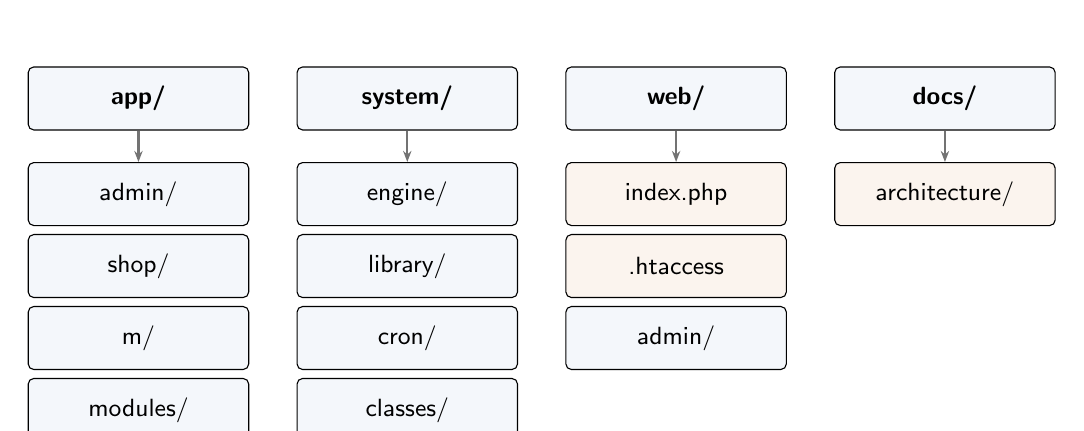
\begin{tikzpicture}[
  dir/.style={draw, rounded corners=2pt, minimum width=2.8cm, minimum height=0.8cm, align=center, font=\small\sffamily, fill=nodefill},
  file/.style={draw, rounded corners=2pt, minimum width=2.8cm, minimum height=0.8cm, align=center, font=\small\sffamily, fill=nodefillalt},
  arr/.style={-{Stealth[length=4pt]}, thick, black!55}
]
  \node[dir] (app) {\textbf{app/}};
  \node[dir, right=0.6cm of app] (system) {\textbf{system/}};
  \node[dir, right=0.6cm of system] (web) {\textbf{web/}};
  \node[dir, right=0.6cm of web] (docs) {\textbf{docs/}};

  \node[dir, below=0.4cm of app] (admin) {admin/};
  \node[dir, below=0.1cm of admin] (shop) {shop/};
  \node[dir, below=0.1cm of shop] (m) {m/};
  \node[dir, below=0.1cm of m] (modules) {modules/};

  \node[dir, below=0.4cm of system] (engine) {engine/};
  \node[dir, below=0.1cm of engine] (library) {library/};
  \node[dir, below=0.1cm of library] (cron) {cron/};
  \node[dir, below=0.1cm of cron] (classes) {classes/};

  \node[file, below=0.4cm of web] (index) {index.php};
  \node[file, below=0.1cm of index] (htaccess) {.htaccess};
  \node[dir, below=0.1cm of htaccess] (adminweb) {admin/};

  \node[file, below=0.4cm of docs] (arch) {architecture/};

  \draw[arr] (app) -- (admin);
  \draw[arr] (system) -- (engine);
  \draw[arr] (web) -- (index);
  \draw[arr] (docs) -- (arch);
\end{tikzpicture}
\caption{Top-level layout of the source tree. Three application
folders (\texttt{app/}, \texttt{system/}, \texttt{web/}) plus the
\texttt{docs/architecture/} folder where this blueprint lives.}
\label{fig:tree-toplevel}
\end{figure}

\subsection{File-Type Breakdown}

\begin{table}[htbp]
\centering
\caption{File-type breakdown of the source commit (12,020 files).}\label{tab:filetypes}
\small
\begin{tabularx}{\columnwidth}{lrX}
\toprule
\textbf{Extension} & \textbf{Count} & \textbf{Role} \\
\midrule
.svg   & 4,607 & Vector theme assets (icons, illustrations) \\
.png   & 3,220 & Raster theme assets (product images, banners, UI chrome) \\
.php   & 1,450 & All application logic: controllers, models, libraries, engine, cron \\
.tpl   & 792   & View templates (per-theme, per-controller) \\
.js    & 676   & Front-end JavaScript (jQuery plugins, theme scripts, admin dashboard) \\
.css   & 220   & Stylesheets (per-theme) \\
.gif   & 176   & Animated theme assets \\
.jpg   & 171   & Photographic theme assets \\
.z     & 84    & Compressed archives (backups, exports) \\
.db    & 24    & SQLite databases (likely caches or local indexes) \\
.html  & 19    & Static HTML fragments \\
.woff / .ttf / .eot / .woff2 & 56 & Web fonts (4 extensions, 14 files each) \\
.md    & 15    & Documentation (including this blueprint's README) \\
.csv   & 15    & Data exports \\
.txt   & 14    & Logs, configs, READMEs \\
.cache & 13    & File-based cache entries \\
.json  & 11    & Package manifests, configs \\
other  & 417   & Logs (\texttt{.log}), code-workspace, \texttt{.htaccess}, \texttt{php.ini}, etc. \\
\bottomrule
\end{tabularx}
\end{table}

The 1,450 PHP files distribute as: \texttt{app/} 1,008 (admin 504,
shop 489, modules 7, m 8 --- though m/ largely re-uses shop/ via
\texttt{DIR\_APPLICATION} redirection), \texttt{system/} 432
(engine 6, library $\sim$50, plus subdirectories), \texttt{web/} 9
(the three entry-point \texttt{index.php} files plus per-app
\texttt{.htaccess} siblings).

\subsection{Three Entry Points, Three Applications}

The source reveals three separate entry points, one per application:

\begin{table}[htbp]
\centering
\caption{The three entry points.}\label{tab:entries}
\small
\begin{tabularx}{\columnwidth}{lllX}
\toprule
\textbf{Entry} & \textbf{App} & \textbf{STORE\_ID} & \textbf{Role} \\
\midrule
\texttt{web/index.php}       & shop & 0 (or detected) & Storefront front controller \\
\texttt{web/admin/index.php} & admin & 0 (hard-coded) & Admin back-office front controller \\
\texttt{web/m/index.php}     & m & 9 (hard-coded) & Mobile entry point (reuses shop/) \\
\bottomrule
\end{tabularx}
\end{table}

All three follow the same shape (config $\to$ startup $\to$ map $\to$
Front::dispatch) but differ in pre-action chain and store scoping.
Section~\ref{sec:bootstrap} walks through \texttt{web/index.php}
line-by-line.

% ============================================================
\section{The Bootstrap Sequence (Verified)}\label{sec:bootstrap}
% ============================================================

\subsection{The Six-Stage Bootstrap}

v1 inferred a 13-phase HTTP request lifecycle from the schema. The
source confirms the broad shape but reveals that the actual bootstrap
is a six-stage sequence spread across four files:

\begin{figure}[htbp]
\centering
\resizebox{\columnwidth}{!}{%
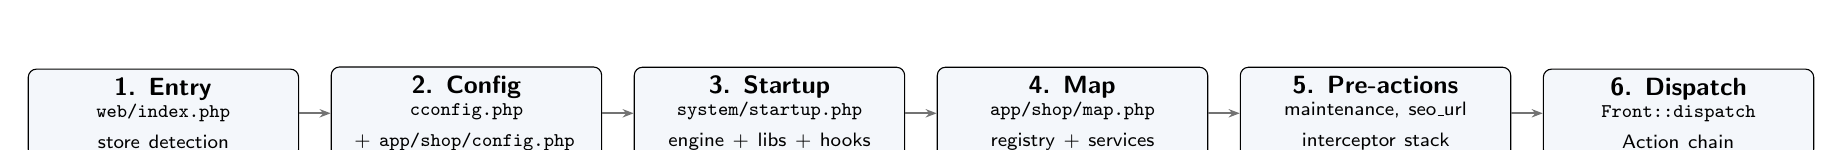
\begin{tikzpicture}[
  stage/.style={draw, rounded corners=3pt, text width=3.2cm, minimum height=1.1cm, align=center, font=\small\sffamily, fill=nodefill},
  arr/.style={-{Stealth[length=4pt]}, thick, black!55}
]
  \node[stage] (s1) {\textbf{1. Entry}\\\scriptsize \texttt{web/index.php}\\\scriptsize store detection};
  \node[stage, right=0.4cm of s1] (s2) {\textbf{2. Config}\\\scriptsize \texttt{cconfig.php}\\\scriptsize + \texttt{app/shop/config.php}};
  \node[stage, right=0.4cm of s2] (s3) {\textbf{3. Startup}\\\scriptsize \texttt{system/startup.php}\\\scriptsize engine + libs + hooks};
  \node[stage, right=0.4cm of s3] (s4) {\textbf{4. Map}\\\scriptsize \texttt{app/shop/map.php}\\\scriptsize registry + services};
  \node[stage, right=0.4cm of s4] (s5) {\textbf{5. Pre-actions}\\\scriptsize maintenance, seo\_url\\\scriptsize interceptor stack};
  \node[stage, right=0.4cm of s5] (s6) {\textbf{6. Dispatch}\\\scriptsize \texttt{Front::dispatch}\\\scriptsize Action chain};

  \draw[arr] (s1) -- (s2);
  \draw[arr] (s2) -- (s3);
  \draw[arr] (s3) -- (s4);
  \draw[arr] (s4) -- (s5);
  \draw[arr] (s5) -- (s6);
\end{tikzpicture}%
}
\caption{The six-stage bootstrap, verified from source. Stage 1
(\texttt{web/index.php}) performs store detection. Stage 2 loads
database credentials and per-app constants. Stage 3 loads the engine
and core libraries. Stage 4 (the misleadingly-named \texttt{map.php})
instantiates the Registry and registers all services. Stage 5 runs
the pre-action interceptor stack. Stage 6 enters the dispatch loop.}
\label{fig:bootstrap}
\end{figure}

\subsection{Stage 1 --- Entry Point and Store Detection}

The actual \texttt{web/index.php} (85 lines) reveals the precise
multi-store detection algorithm --- which v1 could only guess at.

\begin{lstlisting}[caption={Store detection algorithm, abridged from \texttt{web/index.php}.},label={lst:store-detection}]
require_once($config_path . 'cconfig.php');
$db = new mysqli(DB_HOSTNAME, DB_USERNAME, DB_PASSWORD, DB_DATABASE);
if (isset($_GET['_route_'])) {
    $parts = explode("/", $_SERVER['REQUEST_URI']);
    foreach ($parts as $part) {
        if (empty($part)) continue;
        $results = $db->query("SELECT * FROM " . DB_PREFIX . "store WHERE folder = '" . $db->real_escape_string($part) . "'");
        $store = $results->fetch_assoc();
        if ($store['folder']) { $matches[1] = $store['folder']; }
    }
} elseif (isset($_GET['store_id'])) {
    $results = $db->query("SELECT * FROM " . DB_PREFIX . "store WHERE store_id = '" . $db->real_escape_string((int)$_GET['store_id']) . "'");
    $store = $results->fetch_assoc();
    if ($store['store_id']) { $matches[1] = $store['folder']; }
}
if (!isset($matches[1]))
    preg_match('/([^.]+)\.necoyoad\.com/', $_SERVER['SERVER_NAME'], $matches);
if (isset($matches[1]) && $matches[1] != 'www') {
    if (file_exists($config_path . "app/" . strtolower($matches[1]) . "/config.php")) {
        require_once($config_path . "app/" . strtolower($matches[1]) . "/config.php");
    } else {
        require_once($config_path . 'app/shop/config.php');
    }
} else {
    require_once($config_path . 'app/shop/config.php');
}
\end{lstlisting}

Three store-detection strategies, in order:

\begin{enumerate}[leftmargin=1.6em,itemsep=2pt]
  \item \textbf{URL path folder match} --- if \texttt{\_route\_} is
        present, split \texttt{REQUEST\_URI} by \texttt{/} and query
        \texttt{store.folder} for each part. The last matching
        folder wins.
  \item \textbf{Explicit \texttt{?store\_id} GET parameter} ---
        looks up the store by primary key.
  \item \textbf{Subdomain regex} --- a \texttt{preg\_match} call on
        the hostname with a pattern that captures the leftmost label
        (e.g.\ \texttt{m.necoyoad.com} becomes \texttt{m},
        \texttt{foo.necoyoad.com} becomes \texttt{foo}).
\end{enumerate}

After detection, the matching \texttt{app/\{folder\}/config.php} is
required. If no per-store config exists, the system falls back to
\texttt{app/shop/config.php}.

\subsection{Stage 2 --- Config Files}

Three config files fire in sequence:

\begin{itemize}[leftmargin=1.6em,itemsep=2pt]
  \item \texttt{cconfig.php} (root) --- database credentials
        (\texttt{DB\_HOSTNAME}, \texttt{DB\_USERNAME},
        \texttt{DB\_PASSWORD}, \texttt{DB\_DATABASE},
        \texttt{DB\_PREFIX}).
  \item \texttt{app/shop/config.php} --- per-app constants
        (\texttt{STORE\_ID}, \texttt{DIR\_APPLICATION},
        \texttt{DIR\_SYSTEM}, \texttt{DIR\_MODULE}, \texttt{HTTP\_HOME},
        \texttt{HTTP\_ADMIN}, \texttt{HTTP\_IMAGE}, etc.).
  \item \texttt{app/admin/config.php} --- admin overrides (notably
        \texttt{STORE\_ID = 0}, \texttt{ADMIN\_PATH = 'admin'},
        \texttt{DB\_VERSION = '1.0.2'}, \texttt{SYSTEM\_VERSION =
        '1.0.2'}, \texttt{NTS\_DEBUG\_MODE = false}).
\end{itemize}

The version constant \texttt{VERSION = '1.0.2'} (defined in
\texttt{web/index.php} itself) and \texttt{SYSTEM\_VERSION =
'1.0.2'} (defined in \texttt{app/admin/config.php}) confirm that
this is Necoyoad 1.0.2.

\subsection{Stage 3 --- \texttt{system/startup.php}}

\texttt{startup.php} is a 169-line procedural bootstrap that performs
nine things in a fixed order:

\begin{lstlisting}[caption={\texttt{system/startup.php}, the engine bootstrap (abridged).},label={lst:startup}]
// 1. Workflows: load Hooks + Events (the dual extension system)
require_once(DIR_SYSTEM . 'library/automation/hooks.php');
require_once(DIR_SYSTEM . 'library/automation/events.php');
global $hooks;
$hooks = new Hooks("mainstream");

// 2. Error handler (only in debug mode)
if (defined('NTS_DEBUG_MODE') && NTS_DEBUG_MODE === true) {
    set_error_handler('error_handler'); // emits Events::emit("php:error", ...)
}

// 3. Session
require_once(DIR_SYSTEM . 'library/session.php');
$session = new Session();

// 4. Legacy compatibility shims: register_globals, magic_quotes_gpc, IIS DOCUMENT_ROOT
// 5. Engine: Action, Controller, Front, Loader, Model, Registry
require_once(DIR_SYSTEM . 'engine/action.php');
require_once(DIR_SYSTEM . 'engine/controller.php');
require_once(DIR_SYSTEM . 'engine/front.php');
require_once(DIR_SYSTEM . 'engine/loader.php');
require_once(DIR_SYSTEM . 'engine/model.php');
require_once(DIR_SYSTEM . 'engine/registry.php');
Events::emit("engine_load", true);

// 6. Module base class
require_once(DIR_SYSTEM . 'classes/module.php');

// 7. Core libraries
require_once(DIR_SYSTEM . 'library/cache.php');
require_once(DIR_SYSTEM . 'library/config.php');
require_once(DIR_SYSTEM . 'library/db.php');
require_once(DIR_SYSTEM . 'library/document.php');
require_once(DIR_SYSTEM . 'library/language.php');
require_once(DIR_SYSTEM . 'library/log.php');
require_once(DIR_SYSTEM . 'library/request.php');
require_once(DIR_SYSTEM . 'library/response.php');
require_once(DIR_SYSTEM . 'library/url.php');
require_once(DIR_SYSTEM . 'library/image.php');

// 8. Fire the 'init' hook
$hooks->run('init');

// 9. Register a placeholder 'processcss' filter
$hooks->addFilter("processcss", function ($original, $filtered) {
    return $filtered;
});
\end{lstlisting}

Note the ordering: \textbf{the Hooks and Events system loads before
the engine itself}. This is so that the engine classes (Registry,
Loader) can emit events during their own construction.

\subsection{Stage 4 --- \texttt{app/shop/map.php}}

\texttt{map.php} is the most mis-named file in the codebase. It is
\emph{not} a route map and \emph{not} an autoloader configuration.
It is the bootstrap init script that:

\begin{enumerate}[leftmargin=1.6em,itemsep=2pt]
  \item Instantiates the \texttt{Registry}, \texttt{Loader},
        \texttt{Config}, \texttt{DB}, \texttt{Request},
        \texttt{Response}, \texttt{Front} controller.
  \item Loads the \texttt{setting} table into \texttt{Config} (one
        \texttt{SELECT * FROM setting WHERE store\_id = N}, result
        cached in the Config object).
  \item Detects the active language from URL/cookie/session/browser.
  \item Auto-loads platform libraries via \texttt{\$loader->auto(...)}:
        URL, User/Customer, Currency, Tax, Weight, Length, Cart,
        Validar, Encoder, Browser, Tracker.
  \item Registers all services in the Registry.
  \item Fires the \texttt{system\_load}, \texttt{config\_load},
        \texttt{language\_load}, \texttt{app\_load}, and \texttt{load}
        hooks/events.
  \item Detects mobile/tablet/Facebook in-app browsers and either
        redirects or swaps the template.
  \item Loads per-theme \texttt{deps.php} files to register CSS/JS
        dependencies filtered by route.
\end{enumerate}

The admin's \texttt{map.php} (843 lines) additionally runs a giant
\texttt{switch (\$route)} statement that preloads route-specific
model/language/asset dependencies before the controller even
instantiates. The name ``map.php'' derives from this: it literally
maps routes to dependencies.

\subsection{Stage 5 --- Pre-Actions}

\begin{lstlisting}[caption={Pre-action registration in \texttt{web/index.php}.},label={lst:preactions}]
$controller = new Front($registry);
$controller->addPreAction(new Action('common/maintenance/check'));
if ($config->get('config_seo_url')) $controller->addPreAction(new Action('common/seo_url'));
\end{lstlisting}

Pre-actions are an interceptor stack. The storefront registers two:
\texttt{common/maintenance/check} (always) and \texttt{common/seo\_url}
(only if \texttt{config\_seo\_url} is truthy). The admin registers
two different ones: \texttt{common/home/login} (token enforcement)
and \texttt{common/home/permission} (RBAC check). See
Section~\ref{sec:engine} for the dispatch algorithm.

\subsection{Stage 6 --- Dispatch}

\begin{lstlisting}[caption={Dispatch in \texttt{web/index.php}.},label={lst:dispatch}]
if (isset($request->get['r'])) {
    if (!isset($controller->ClassName)) $controller->ClassName = $request->get['r'];
    $action = new Action($request->get['r']);
} else {
    $action = new Action('common/home');
}
$controller->dispatch($action, new Action('error/not_found'));
$response->output();
\end{lstlisting}

The route parameter is \texttt{?r=}, not OpenCart's \texttt{?route=}.
If absent, the default route is \texttt{common/home}. The error
fallback is \texttt{error/not\_found}.

% ============================================================
\section{The Engine (Verified)}\label{sec:engine}
% ============================================================

The engine lives in \texttt{system/engine/} and consists of six
classes: \texttt{Registry}, \texttt{Action}, \texttt{Front},
\texttt{Controller}, \texttt{Loader}, \texttt{Model}. Together they
form the OpenCart-derived MVC spine that Necoyoad inherits.

\subsection{Registry --- Service Locator}

\begin{lstlisting}[caption={\texttt{system/engine/registry.php} --- the entire class.},label={lst:registry}]
final class Registry {
    private $data = array();

    public function get($key) {
        return (isset($this->data[$key]) ? $this->data[$key] : null);
    }

    public function set($key, $value) {
        if (class_exists("Events") && is_callable([Events::class, 'emit'])) {
            Events::emit(strtolower(__CLASS__).":update", $key, $value);
        }
        $this->data[$key] = $value;
    }

    public function has($key) {
        return isset($this->data[$key]);
    }
}
\end{lstlisting}

A textbook Registry/Service Locator. Only one instance exists per
request. Every long-lived service (\texttt{db}, \texttt{config},
\texttt{request}, \texttt{response}, \texttt{session},
\texttt{customer}, \texttt{cart}, \texttt{tax}, \texttt{currency},
\texttt{user}, \texttt{load}, \texttt{cache}, \texttt{log},
\texttt{language}, \texttt{url}, \texttt{document}, \texttt{image},
\texttt{tracker}, \texttt{mailer}) is parked here, and every
controller/model/lib accesses it through the \texttt{\_\_get}/\texttt{\_\_set}
proxies on \texttt{Controller}, \texttt{Model}, \texttt{Loader},
\texttt{Cart}, etc.

Notable: \texttt{set()} emits \texttt{Events::emit("registry:update",
\$key, \$value)} if the Events system is available. The Registry is
\emph{observable} --- listeners can react whenever a service is
parked. This is what allows Necoyoad modules to spy on each other's
registered services.

\subsection{Action --- Route Resolver}

The \texttt{Action} class is the dispatch token. Given a route
string like \texttt{common/home} or \texttt{store/product}, it
resolves the file, class, and method to invoke.

\begin{lstlisting}[caption={\texttt{system/engine/action.php} --- route resolution algorithm (abridged).},label={lst:action}]
final class Action {
    public $route;
    private $file, $class, $method, $args = array();

    public function __construct($route, $args = array()) {
        $this->route = $route;
        $path = '';
        $parts = explode('/', str_replace('../', '', $route));
        $default_path = DIR_APPLICATION;

        // Module route: modules/<module>/<app>/<controller>/<method>
        if ($parts[0] === 'modules') {
            $module = $parts[1];
            $default_path = DIR_MODULE . $module . '/app/';
            array_shift($parts); // consume 'modules'
            array_shift($parts); // consume module name
            // next part is the app (shop, admin)
            array_shift($parts);
        }

        // Walk parts: each part is either a directory or a file
        foreach ($parts as $part) {
            $path .= $part;
            if (is_dir($default_path . 'controller/' . $path)) {
                $path .= '/';
                array_shift($parts);
                continue;
            }
            if (is_file($default_path . 'controller/' . str_replace('../', '', $path) . '.php')) {
                $this->file  = $default_path . 'controller/' . str_replace('../', '', $path) . '.php';
                $this->class = 'Controller' . preg_replace('/[^a-zA-Z0-9]/', '', $path);
                array_shift($parts);
                break;
            }
            array_shift($parts);
        }

        $method = array_shift($parts);
        if ($method) { $this->method = $method; } else { $this->method = 'index'; }
    }
}
\end{lstlisting}

The resolution algorithm is purely string-convention based --- no
annotations, no DI introspection. Concrete examples:

\begin{table}[htbp]
\centering
\caption{Action route resolution (verified from source).}\label{tab:action-resolution}
\footnotesize\sloppy
\resizebox{\columnwidth}{!}{%
\begin{tabular}{llll}
\toprule
\textbf{Route} & \textbf{File} & \textbf{Class} & \textbf{Method} \\
\midrule
\texttt{common/home}              & \texttt{controller/common/home.php}        & \texttt{ControllerCommonHome}        & \texttt{index} \\
\texttt{store/product}            & \texttt{controller/store/product.php}      & \texttt{ControllerStoreProduct}      & \texttt{index} \\
\texttt{store/manufacturer/index} & \texttt{controller/store/manufacturer.php} & \texttt{ControllerStoreManufacturer} & \texttt{index} \\
\texttt{checkout/cart}            & \texttt{controller/checkout/cart.php}      & \texttt{ControllerCheckoutCart}      & \texttt{index} \\
\texttt{api/v1/products}          & \texttt{controller/api/v1.php}             & \texttt{ControllerApiV1}             & \texttt{products} \\
\texttt{modules/mymodule/shop/home} & \texttt{DIR\_MODULE . mymodule/app/shop/controller/home.php} & \texttt{ControllerHome} & \texttt{index} \\
\bottomrule
\end{tabular}%
}
\end{table}

The same route string (\texttt{common/home}) dispatches to
\emph{different files} depending on which \texttt{DIR\_APPLICATION}
is currently set. The class name is \texttt{Controller} + the
uppercase-first of each path segment concatenated.

\subsection{Front --- Front Controller and Dispatch Loop}

\begin{lstlisting}[caption={\texttt{system/engine/front.php} --- the dispatch loop.},label={lst:front}]
final class Front {
    private $registry, $pre_action = array(), $error;

    public function __construct($registry) { $this->registry = $registry; }

    public function addPreAction($pre_action) { $this->pre_action[] = $pre_action; }

    public function dispatch($action, $error) {
        $this->error = $error;
        // Pre-actions: first truthy return replaces the main action
        foreach ($this->pre_action as $pre_action) {
            $result = $this->execute($pre_action);
            Events::emit("dispatch", $pre_action);
            if ($result) { $action = $result; break; }
        }
        // Main action loop: continues as long as controllers return new Actions
        while ($action) {
            Events::emit("dispatch", $action);
            $action = $this->execute($action);
        }
    }

    private function execute($action) {
        if ($action) {
            // Register routing context into the registry
            if (!empty($action->route)) {
                $this->registry->set('ClassName', $action->class);
                $this->registry->set('Method',    $action->method);
                $this->registry->set('Route',     $action->route);
            }
            if (file_exists($action->getFile())) {
                require_once($action->getFile());
                $controller = new $action->getClass()($this->registry);
                if (is_callable(array($controller, $action->getMethod()))) {
                    $action = call_user_func_array(array($controller, $action->getMethod()), $action->getArgs());
                } else {
                    $action = $this->error;
                    $this->error = '';
                }
            } else {
                $action = $this->error;
                $this->error = '';
            }
        }
        return $action;
    }
}
\end{lstlisting}

The dispatch algorithm has three notable properties:

\begin{enumerate}[leftmargin=1.6em,itemsep=2pt]
  \item \textbf{Pre-actions are an interceptor stack.} The first
        pre-action that returns a truthy value replaces the main
        action and breaks the pre-action loop. This is how
        \texttt{common/maintenance/check} can short-circuit to the
        maintenance page, and how \texttt{common/seo\_url} rewrites
        \texttt{\_route\_} into a \texttt{?r=} value.
  \item \textbf{Controllers forward by returning new Actions.} The
        main loop continues as long as controllers return new
        \texttt{Action} objects. This is controller-to-controller
        forwarding.
  \item \textbf{Error handling is one-shot.} The error action is
        invoked at most once; after that \texttt{\$this->error = ''}
        prevents infinite loops.
\end{enumerate}

\subsection{Controller --- Abstract Base}

The \texttt{Controller} base class provides:

\begin{itemize}[leftmargin=1.6em,itemsep=2pt]
  \item \texttt{\_\_get(\$key)} / \texttt{\_\_set(\$key, \$value)} ---
        delegate to \texttt{\$this->registry->get/set}. This is how
        controllers magically access \texttt{\$this->db},
        \texttt{\$this->config}, \texttt{\$this->request}, etc.
  \item \texttt{get(\$key)} / \texttt{set(\$key, \$value)} ---
        read/write the view-model \texttt{\$this->data[]}.
  \item \texttt{on(\$ev, \$fn)} $\to$ \texttt{Events::on(\$ev, \$fn)}
  \item \texttt{off(\$ev)} $\to$ \texttt{Events::off(\$ev)}
  \item \texttt{trigger(\$ev, ...\$args)} $\to$
        \texttt{Events::emit(\$ev, \$args)}
  \item \texttt{addFilter(\$name, \$fn)} $\to$
        \texttt{\$hooks->addFilter(\$this->namespace . \$name, \$fn)}
        (namespaced)
  \item \texttt{applyFilters(\$name, \$value)} $\to$
        \texttt{\$hooks->applyFilters(\$name, \$value)}
  \item \texttt{addHook(\$name, \$fn)} $\to$
        \texttt{\$hooks->addAction(\$name, \$fn)}
  \item \texttt{runHook(\$name, ...\$args)} $\to$
        \texttt{\$hooks->run(\$name, \$args)}
  \item \texttt{setvar(\$varname, \$model, \$default)} --- sets a
        view variable with a 5-level priority fallback:
        \texttt{\$\_POST[\$varname]} $\to$
        \texttt{\$model[\$varname]} $\to$
        \texttt{\$\_GET[\$varname]} $\to$
        \texttt{config->get(\$varname)} $\to$
        \texttt{\$default} $\to$ \texttt{''}.
  \item \texttt{forward(\$route, \$args)} --- returns a new
        \texttt{Action(\$route, \$args)} (controller-to-controller
        forwarding).
  \item \texttt{redirect(\$url)} --- runs the \texttt{redirect} hook;
        if no hook returns truthy, emits the \texttt{redirect} event,
        then either \texttt{header('Location: ...') + exit} or, if
        headers already sent, an inline
        \texttt{<script>window.location=...</script>}.
  \item \texttt{addChild(\$child, \$params)} /
        \texttt{getChild} / \texttt{getChildren} --- composite-view
        pattern (header/footer/column children).
  \item \texttt{render()} --- renders the template, then renders
        children, then applies the \texttt{fetch} hook.
  \item \texttt{fetch(\$template)} --- loads the template file,
        extracts \texttt{\$this->data} into local variables, runs
        \texttt{applyFilters("fetch", ...)}.
  \item \texttt{loadWidgets()} / \texttt{loadAssets()} --- widget
        substitution and asset loading.
\end{itemize}

The dual Hooks/Events bridge is built into the controller base: every
controller subclass can register both Hooks (WordPress-style filters
and actions, namespaced) and Events (Node-style observers) without
loading any additional dependencies.

\subsection{Loader --- Lazy Resource Loader}

\begin{lstlisting}[caption={\texttt{system/engine/loader.php} --- model loading (abridged).},label={lst:loader}]
final class Loader {
    private $registry;

    public function __construct($registry) { $this->registry = $registry; }

    public function model($model) {
        $key = 'model_' . str_replace('/', '_', $model);
        $legacy_key = 'model_' . str_replace('/', '_', preg_replace('/[^a-zA-Z0-9_\/]/', '', $model));
        if (!$this->registry->has($key) && !$this->registry->has($legacy_key)) {
            $file = DIR_MODEL . $model . '.php';
            $class = 'Model' . preg_replace('/[^a-zA-Z0-9]/', '', $model);
            if (file_exists($file)) {
                require_once($file);
                $instance = new $class($this->registry);
                $this->registry->set($key, $instance);
                $this->registry->set($legacy_key, $instance); // legacy alias
            }
        }
    }

    public function library($library) { /* include_once DIR_SYSTEM . 'library/' . $library . '.php' */ }
    public function helper($helper)   { /* include_once DIR_SYSTEM . 'helper/' . $helper . '.php' */ }
    public function auto($class)      { /* library + instantiate + register in Registry */ }
}
\end{lstlisting}

Each model is loaded once per request and registered under two
registry keys: the canonical \texttt{model\_<path>} and a legacy
\texttt{model\_<path>} alias. Controllers access models as
\texttt{\$this->model\_checkout\_order} via the Registry
\texttt{\_\_get} proxy.

\subsection{Model --- Active-Record-ish Base with Hookable CRUD}

\begin{lstlisting}[caption={\texttt{system/engine/model.php} --- the CRUD bridge (abridged).},label={lst:model}]
abstract class Model {
    protected $registry;

    public function __construct($registry) { $this->registry = $registry; }

    public function __get($key) { return $this->registry->get($key); }
    public function __set($key, $value) { $this->registry->set($key, $value); }

    // Hook bridges
    public function addHook($name, $fn) { /* $hooks->addAction(...) */ }
    public function runHook($name, ...$args) { /* $hooks->run(...) */ }
    public function addFilter($name, $fn) { /* $hooks->addFilter(...) */ }
    public function applyFilters($name, $value) { /* $hooks->applyFilters(...) */ }

    // Generic CRUD: subclasses set $table, $pk, $fields
    public function add($data)        { /* INSERT ... */ }
    public function update($id, $data){ /* UPDATE ... */ }
    public function delete($id)       { /* DELETE ... */ }
    public function getById($id)      { /* SELECT ... */ }
    public function getAll($filters)  { /* SELECT with buildSQLQuery */ }

    protected function buildSQLQuery($filters) {
        // Hand-builds SQL from $filters array
        // Each filter can be: eq, neq, gt, gte, lt, lte, like, in, between, null, notnull
        // Returns: [SQL string, params array]
    }

    // EAV property bridge (the `property` table)
    public function getProperty($object_id, $group, $key) { /* ... */ }
    public function setProperty($object_id, $group, $key, $value) { /* ... */ }
    public function deleteProperty($object_id, $group, $key) { /* ... */ }
    public function getAllProperties($object_id, $group = null) { /* ... */ }
}
\end{lstlisting}

The \texttt{Model} base provides generic CRUD that subclasses can
override. The \texttt{buildSQLQuery} method is a hand-built query
constructor that supports filter operators \texttt{eq, neq, gt, gte,
lt, lte, like, in, between, null, notnull}. The
\texttt{setProperty}/\texttt{getProperty} methods are the bridge to
the polymorphic EAV \texttt{property} table.

% ============================================================
\section{The Dual Hooks/Events Extension System}\label{sec:hooks}
% ============================================================

One of the most architecturally significant findings the source
reveals is that Necoyoad has \textbf{two parallel extension systems}
that coexist throughout the codebase:

\begin{itemize}[leftmargin=1.6em,itemsep=2pt]
  \item \textbf{Hooks} --- WordPress-style filters and actions.
        \texttt{addFilter}, \texttt{applyFilters}, \texttt{addAction},
        \texttt{run}. Filters short-circuit on truthy return.
  \item \textbf{Events} --- Node-style observer pattern.
        \texttt{on}, \texttt{emit}, \texttt{off}, \texttt{once}.
        No short-circuit; all listeners always fire.
\end{itemize}

\subsection{Hooks (WordPress-style)}

\begin{lstlisting}[caption={\texttt{system/library/automation/hooks.php} --- the Hooks class (abridged).},label={lst:hooks}]
class Hooks {
    private $name;        // namespace ("mainstream")
    private $actions = [];  // registered action callables
    private $filters = [];  // registered filter callables

    public function __construct($name) { $this->name = $name; }

    public function addAction($name, $callable) {
        $this->actions[$name][] = $callable;
    }

    public function run($name, $args = []) {
        if (!isset($this->actions[$name])) return false;
        foreach ($this->actions[$name] as $callable) {
            $result = call_user_func_array($callable, $args);
            if ($result) return $result; // short-circuit on truthy
        }
        return false;
    }

    public function addFilter($name, $callable) {
        $this->filters[$name][] = $callable;
    }

    public function applyFilters($name, $value, ...$extra) {
        if (!isset($this->filters[$name])) return $value;
        foreach ($this->filters[$name] as $callable) {
            $value = call_user_func($callable, $value, ...$extra);
        }
        return $value;
    }
}
\end{lstlisting}

The Hooks system follows WordPress's pattern precisely: actions are
side-effect callbacks that short-circuit on truthy return; filters
chain a value through a series of transforms. Hooks are namespaced
(by the \texttt{\$name} constructor argument, ``mainstream'' by
default) and Controller subclasses further namespace filter names
with \texttt{\$this->namespace}.

\subsection{Events (Node-style)}

\begin{lstlisting}[caption={\texttt{system/library/automation/events.php} --- the Events class (abridged).},label={lst:events}]
class Events {
    private static $listeners = [];

    public static function on($event, $callable) {
        self::$listeners[$event][] = $callable;
    }

    public static function once($event, $callable) {
        $wrapper = function (...$args) use (&$wrapper, $event, $callable) {
            Events::off($event, $wrapper);
            return call_user_func_array($callable, $args);
        };
        self::on($event, $wrapper);
    }

    public static function emit($event, ...$args) {
        if (!isset(self::$listeners[$event])) return;
        foreach (self::$listeners[$event] as $callable) {
            call_user_func_array($callable, $args);
            // no short-circuit: all listeners always fire
        }
    }

    public static function off($event, $callable = null) {
        if ($callable === null) {
            unset(self::$listeners[$event]);
        } else {
            // remove specific callable
        }
    }
}
\end{lstlisting}

Events is a static class with a single global listener registry. It
follows Node's \texttt{EventEmitter} pattern: \texttt{on} subscribes,
\texttt{emit} fires all listeners in order, \texttt{off} unsubscribes.
There is no short-circuit; every listener always runs.

\subsection{When to Use Which}

The codebase uses Hooks and Events for different purposes:

\begin{table}[htbp]
\centering
\caption{Hooks vs Events usage patterns in the codebase.}\label{tab:hooks-vs-events}
\small
\begin{tabularx}{\columnwidth}{llX}
\toprule
\textbf{System} & \textbf{Use case} & \textbf{Examples in source} \\
\midrule
Hooks (filters) & Transform a value through a chain & \texttt{processcss}, \texttt{fetch}, \texttt{data:update}, \texttt{query} (intercept any DB query) \\
Hooks (actions) & Short-circuit a flow with a side effect & \texttt{init}, \texttt{redirect}, \texttt{system\_load}, \texttt{config\_load}, \texttt{language\_load} \\
Events & Broadcast that something happened & \texttt{engine\_load}, \texttt{dispatch}, \texttt{registry:update}, \texttt{php:error}, \texttt{error} \\
\bottomrule
\end{tabularx}
\end{table}

The two systems are not redundant --- they serve different needs.
Hooks are for \emph{transforming} values and \emph{short-circuiting}
flows. Events are for \emph{broadcasting} occurrences. A module that
wants to modify the rendered HTML uses a Hook filter on
\texttt{fetch}; a module that wants to log every dispatch uses an
Event listener on \texttt{dispatch}.

\subsection{Notable Event/Hook Emit Points}

The source fires events at every major lifecycle point:

\begin{table}[htbp]
\centering
\caption{Selected event/hook emit points in the source.}\label{tab:emit-points}
\small
\begin{tabularx}{\columnwidth}{llX}
\toprule
\textbf{Emit point} & \textbf{Type} & \textbf{When} \\
\midrule
\texttt{init} & Hook (action) & End of \texttt{startup.php} \\
\texttt{engine\_load} & Event & After engine classes load \\
\texttt{system\_load} & Hook + Event & \texttt{map.php}, after Registry/DB/Loader/Config construct \\
\texttt{config\_load} & Hook + Event & After \texttt{setting} table loaded into Config \\
\texttt{language\_load} & Hook + Event & After language files load \\
\texttt{app\_load} & Hook + Event & After all libraries auto-loaded \\
\texttt{load} & Hook + Event & End of \texttt{map.php} bootstrap \\
\texttt{dispatch} & Event & Around every Action dispatch \\
\texttt{registry:update} & Event & Every \texttt{Registry::set()} call \\
\texttt{redirect} & Hook + Event & On \texttt{Controller::redirect()} \\
\texttt{fetch} & Hook (filter) & When a template is fetched \\
\texttt{data:update} & Hook (filter) & When a view-model variable is set \\
\texttt{query} & Hook (filter) & Every \texttt{DB::query()} call \\
\texttt{processcss} & Hook (filter) & CSS processing pipeline \\
\texttt{php:error} & Event & PHP error in debug mode \\
\texttt{error} & Event & Same as \texttt{php:error}, generic alias \\
\bottomrule
\end{tabularx}
\end{table}

The \texttt{query} filter is particularly powerful: any module can
intercept any SQL query the application issues, by registering a
filter on \texttt{query}. This is the foundation of Necoyoad's
module ecosystem.

% ============================================================
\section{The 13-Phase HTTP Request Lifecycle (Verified)}\label{sec:lifecycle-v2}
% ============================================================

v1 inferred a 13-phase HTTP request lifecycle from the schema. The
source verifies the broad shape but reveals that several phases
happen in a different order than v1 guessed, and that there are
sub-phases within the bootstrap. The verified lifecycle:

\begin{figure}[htbp]
\centering
\resizebox{\columnwidth}{!}{%
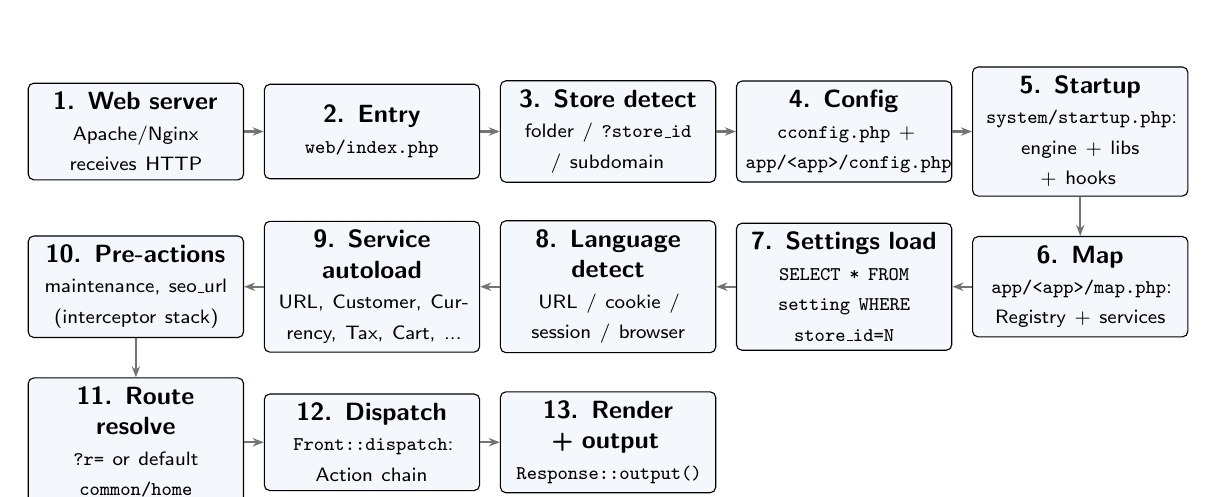
\begin{tikzpicture}[
  phase/.style={draw, rounded corners=2pt, text width=2.5cm, minimum height=1.2cm, align=center, font=\small\sffamily, fill=nodefill},
  arr/.style={-{Stealth[length=4pt]}, thick, black!55}
]
  \node[phase] (p1) {\textbf{1. Web server}\\\scriptsize Apache/Nginx receives HTTP};
  \node[phase, right=0.25cm of p1] (p2) {\textbf{2. Entry}\\\scriptsize \texttt{web/index.php}};
  \node[phase, right=0.25cm of p2] (p3) {\textbf{3. Store detect}\\\scriptsize folder / \texttt{?store\_id} / subdomain};
  \node[phase, right=0.25cm of p3] (p4) {\textbf{4. Config}\\\scriptsize \texttt{cconfig.php} + \texttt{app/<app>/config.php}};
  \node[phase, right=0.25cm of p4] (p5) {\textbf{5. Startup}\\\scriptsize \texttt{system/startup.php}: engine + libs + hooks};

  \node[phase, below=0.5cm of p5] (p6) {\textbf{6. Map}\\\scriptsize \texttt{app/<app>/map.php}: Registry + services};
  \node[phase, left=0.25cm of p6] (p7) {\textbf{7. Settings load}\\\scriptsize \texttt{SELECT * FROM setting WHERE store\_id=N}};
  \node[phase, left=0.25cm of p7] (p8) {\textbf{8. Language detect}\\\scriptsize URL / cookie / session / browser};
  \node[phase, left=0.25cm of p8] (p9) {\textbf{9. Service autoload}\\\scriptsize URL, Customer, Currency, Tax, Cart, ...};
  \node[phase, left=0.25cm of p9] (p10) {\textbf{10. Pre-actions}\\\scriptsize maintenance, seo\_url (interceptor stack)};

  \node[phase, below=0.5cm of p10] (p11) {\textbf{11. Route resolve}\\\scriptsize \texttt{?r=} or default \texttt{common/home}};
  \node[phase, right=0.25cm of p11] (p12) {\textbf{12. Dispatch}\\\scriptsize \texttt{Front::dispatch}: Action chain};
  \node[phase, right=0.25cm of p12] (p13) {\textbf{13. Render + output}\\\scriptsize \texttt{Response::output()}};

  \draw[arr] (p1) -- (p2);
  \draw[arr] (p2) -- (p3);
  \draw[arr] (p3) -- (p4);
  \draw[arr] (p4) -- (p5);
  \draw[arr] (p5) -- (p6);
  \draw[arr] (p6) -- (p7);
  \draw[arr] (p7) -- (p8);
  \draw[arr] (p8) -- (p9);
  \draw[arr] (p9) -- (p10);
  \draw[arr] (p10) -- (p11);
  \draw[arr] (p11) -- (p12);
  \draw[arr] (p12) -- (p13);
\end{tikzpicture}%
}
\caption{The verified 13-phase HTTP request lifecycle. Phases 5--9
are the bootstrap stages identified in
Figure~\ref{fig:bootstrap}, expanded. Phase 10 runs the pre-action
interceptor stack. Phase 11 resolves the route (either from
\texttt{?r=} or from the SEO URL rewriter). Phase 12 is the dispatch
loop. Phase 13 renders and outputs.}
\label{fig:lifecycle-v2}
\end{figure}

\subsection{Phase Notes (Verified)}

\begin{description}[leftmargin=1.6em,itemsep=2pt,font=\bfseries\small]
  \item[Phase 3 --- Store detect:] Three strategies in fixed order:
        URL path folder match, \texttt{?store\_id} GET param,
        subdomain regex. Verified in \texttt{web/index.php} lines
        21--42 (Listing~\ref{lst:store-detection}).
  \item[Phase 5 --- Startup:] Loads Hooks + Events first, then
        engine, then core libraries. Fires \texttt{init} hook at the
        end. Verified in \texttt{system/startup.php}
        (Listing~\ref{lst:startup}).
  \item[Phase 6 --- Map:] Instantiates Registry and core services.
        Misleadingly named; it is a bootstrap init script, not a
        route map. Fires \texttt{system\_load}, \texttt{config\_load},
        \texttt{language\_load}, \texttt{app\_load}, and \texttt{load}
        events.
  \item[Phase 7 --- Settings load:] A single
        \texttt{SELECT * FROM setting WHERE store\_id = N} query.
        Result rows are pushed into \texttt{Config::set(\$key,
        \$value)}. Subsequent \texttt{\$config->get(...)} calls are
        pure array lookups --- no further DB hits.
  \item[Phase 8 --- Language detect:] Storefront detects from URL
        (first path segment), then cookie, then session, then
        \texttt{HTTP\_ACCEPT\_LANGUAGE} browser header. Admin uses
        \texttt{config\_admin\_language} setting.
  \item[Phase 9 --- Service autoload:] \texttt{\$loader->auto(...)}
        instantiates each service and registers it in the Registry.
        Customer is loaded eagerly by \texttt{customer\_id} from
        session (if logged in). Cart is loaded from the file cache
        (keyed by \texttt{customer\_id ?? session\_id}).
  \item[Phase 10 --- Pre-actions:] The interceptor stack runs.
        \texttt{common/maintenance/check} runs first; if maintenance
        mode is on and visitor is not admin, it short-circuits to the
        maintenance page. \texttt{common/seo\_url} runs second;
        rewrites \texttt{\_route\_} into \texttt{?r=} (see
        Section~\ref{sec:seo-source}).
  \item[Phase 11 --- Route resolve:] If \texttt{?r=} is set, that is
        the route. Otherwise the default is \texttt{common/home}.
  \item[Phase 12 --- Dispatch:] \texttt{Front::dispatch} runs the
        pre-action stack, then the main action loop. Controllers can
        forward by returning new \texttt{Action} objects. Error
        action is \texttt{error/not\_found}, fires at most once.
  \item[Phase 13 --- Render + output:] \texttt{Controller::render()}
        loads the template, extracts \texttt{\$this->data} into
        local variables, applies the \texttt{fetch} filter, renders
        children, and returns the output.
        \texttt{Response::output()} sends it to the browser.
\end{description}

% ============================================================
\section{Authentication and Password Algorithm (Corrected)}\label{sec:auth}
% ============================================================

v1 inferred from the 100-character \texttt{customer.password} column
that the system used bcrypt or argon2. The source reveals this is
incorrect.

\subsection{The Actual Password Algorithm}

\begin{lstlisting}[caption={\texttt{system/library/customer.php} --- the actual login method (abridged).},label={lst:customer-login}]
public function login($email, $password, $hash = true) {
    if (empty($email) || empty($password)) return false;

    if ($hash) {
        $password = md5($password);     // MD5 of plaintext
    }

    $query = $this->db->query("SELECT `password` FROM " . DB_PREFIX . "customer
        WHERE `email` = '" . $this->db->escape($email) . "'");
    list($pass, $suffix) = explode(':', $query->row['password']);

    if (!$suffix) {
        // Lazy salt migration: generate a random suffix and re-hash
        $suffix = md5(base_convert(rand(10e16, 10e20), 10, 36) . time());
        $this->db->query("UPDATE " . DB_PREFIX . "customer SET
          `password` = '" . $this->db->escape(md5($password . $suffix) . ':' . $suffix) . "'
          WHERE `email` = '" . $this->db->escape($email) . "'");
    }

    $customer_query = $this->db->query("SELECT * FROM " . DB_PREFIX . "customer WHERE
        email = '" . $this->db->escape($email) . "'
        AND password = '" . $this->db->escape(md5($password . $suffix) . ':' . $suffix) . "'
        AND status = '1'
        AND banned = '0'");
    // ... if found, set session, update visits + ip, merge cart ...
}
\end{lstlisting}

The password storage format is:

\begin{equation*}
\texttt{password} = \underbrace{\text{md5}(\text{md5}(\text{plaintext}) \cdot \text{suffix})}_{32\text{ chars}} \;\cdot\;\texttt{:}\;\cdot\; \underbrace{\text{suffix}}_{32\text{ chars}}
\end{equation*}

i.e.\ \textbf{double-MD5 with a per-row random salt}. The
\texttt{suffix} is a 32-character MD5 hex string. The full stored
password is $32 + 1 + 32 = 65$ characters; the 100-character column
width inferred by v1 is more than enough headroom but is
\emph{not} indicative of bcrypt (60 chars) or argon2id (97+ chars).

\subsection{Lazy Salt Migration}

Notable in Listing~\ref{lst:customer-login} is the lazy salt
migration: if a customer row's \texttt{password} column does not
contain a \texttt{:} separator (i.e.\ it was stored in an older
format without a salt), the system generates a random suffix,
re-hashes the password with it, and updates the row. This means the
system can be upgraded from an unsalted-MD5 scheme to the
salted-double-MD5 scheme one login at a time, without a bulk
migration.

The same algorithm is used for admin users in
\texttt{system/library/user.php} (same code, different table name).

\subsection{OAuth Login}

The source also reveals an OAuth layer that v1 could not see. The
\texttt{Customer} library has OAuth login methods for five providers:
Facebook, Google, Twitter, MercadoLibre (meli), and a generic OAuth2.
These set \texttt{\$\_SESSION['customer\_id']} directly after
verifying the provider's OAuth callback, bypassing the password
check entirely.

\subsection{Permission Model (Verified)}

v1's inference about the admin permission model was correct. The
source confirms:

\begin{itemize}[leftmargin=1.6em,itemsep=2pt]
  \item \texttt{user\_group.permission} is a serialised PHP array
        with \texttt{access} and \texttt{modify} keys, each
        containing a list of route strings.
  \item The admin's two pre-actions enforce auth:
        \texttt{common/home/login} (session token check) and
        \texttt{common/home/permission} (RBAC check).
  \item The \texttt{permission} check reads the current route from
        \texttt{\$request->get['r']}, and depending on the HTTP
        method, checks \texttt{access} (for GET) or \texttt{modify}
        (for POST/PUT/DELETE) in the user's group
        \texttt{permission} blob.
  \item The schema allows additional keys (\texttt{create},
        \texttt{delete}, etc.) which some modules use.
\end{itemize}

% ============================================================
\section{The Order Creation Flow (Verified)}\label{sec:order-flow}
% ============================================================

v1 reconstructed a 9-step order-placement flow from the schema. The
source confirms all 9 steps and adds a 0th step that v1 could not
have known about: garbage collection of abandoned orders.

\subsection{Step 0 --- Garbage Collection}

\begin{lstlisting}[caption={\texttt{app/shop/model/checkout/order.php::create()} --- the garbage-collection step.},label={lst:order-gc}]
// Step 0: garbage-collect abandoned orders (older than 1 month, status = 0)
$query = $this->db->query("SELECT order_id
    FROM `" . DB_PREFIX . "order`
    WHERE date_added < '" . date('Y-m-d', strtotime('-1 month')) . "'
    AND order_status_id = '0'");

foreach ($query->rows as $result) {
    $this->db->query("DELETE FROM `" . DB_PREFIX . "order` WHERE order_id = '" . (int)$result['order_id'] . "'");
    $this->db->query("DELETE FROM " . DB_PREFIX . "order_history WHERE order_id = '" . (int)$result['order_id'] . "'");
    $this->db->query("DELETE FROM " . DB_PREFIX . "order_product WHERE order_id = '" . (int)$result['order_id'] . "'");
    $this->db->query("DELETE FROM " . DB_PREFIX . "order_option WHERE order_id = '" . (int)$result['order_id'] . "'");
    $this->db->query("DELETE FROM " . DB_PREFIX . "order_download WHERE order_id = '" . (int)$result['order_id'] . "'");
    $this->db->query("DELETE FROM " . DB_PREFIX . "order_total WHERE order_id = '" . (int)$result['order_id'] . "'");
}
\end{lstlisting}

Every time \texttt{create()} is called, it first deletes all orders
older than 1 month that still have \texttt{order\_status\_id = 0}
(the initial ``pending'' status set by \texttt{create()} itself).
This is the cleanup of unconfirmed carts --- orders that were
created but never confirmed by the customer.

\subsection{Steps 1--5 --- The Order INSERT}

After garbage collection, \texttt{create()} performs the 5-step
insertion v1 reconstructed:

\begin{enumerate}[leftmargin=1.6em,itemsep=2pt]
  \item \textbf{INSERT the \texttt{order} row} with all denormalised
        customer/shipping/payment fields (30+ columns including
        \texttt{store\_name}, \texttt{store\_url},
        \texttt{customer\_id}, \texttt{firstname}, \texttt{lastname},
        \texttt{email}, \texttt{telephone}, \texttt{total},
        \texttt{language\_id}, \texttt{currency}, \texttt{coupon\_id},
        \texttt{ip}, \texttt{order\_status\_id},
        \texttt{shipping\_*}, \texttt{payment\_*}). The
        \texttt{order\_status\_id} is set to
        \texttt{config\_order\_status\_id} (the ``pending'' status).
  \item \textbf{INSERT \texttt{order\_product} rows} --- one per
        cart line, with snapshot of \texttt{name}, \texttt{model},
        \texttt{price}, \texttt{total}, \texttt{tax},
        \texttt{quantity}.
  \item \textbf{INSERT \texttt{order\_option} rows} --- for each
        product's selected options (variant choices).
  \item \textbf{Set EAV properties} for each product attribute ---
        order attributes are stored in the polymorphic
        \texttt{property} table under group
        \texttt{product\_attribute}, via \texttt{\$this->setProperty(\$order\_id,
        'product\_attribute', \$key, \$value)}.
  \item \textbf{INSERT \texttt{order\_download} rows} --- for each
        digital download attached to a product.
  \item \textbf{INSERT \texttt{order\_total} rows} --- one per
        computed total line (\texttt{title}, \texttt{text},
        \texttt{value}, \texttt{sort\_order}).
\end{enumerate}

\subsection{The \texttt{confirm()} Method}

\texttt{create()} does \emph{not} confirm the order --- it leaves it
in \texttt{order\_status\_id = pending}. Confirmation is a separate
method, \texttt{confirm(\$order\_id, \$order\_status\_id,
\$comment)}, which:

\begin{enumerate}[leftmargin=1.6em,itemsep=2pt]
  \item \textbf{Lock check} --- only proceeds if
        \texttt{order.order\_status\_id = 0} (i.e.\ unconfirmed).
        This makes \texttt{confirm()} idempotent.
  \item \textbf{UPDATE the order status} to the new
        \texttt{order\_status\_id}.
  \item \textbf{INSERT into \texttt{order\_history}} --- the audit
        trail row, with \texttt{notify = 1}.
  \item \textbf{Decrement product stock} --- for each
        \texttt{order\_product} row where \texttt{product.subtract =
        1}, decrement \texttt{product.quantity}. Also decrement
        \texttt{product\_option\_value.quantity} for variant stock.
        Clears the \texttt{product} cache afterwards.
\end{enumerate}

\subsection{Verification of v1's 9-Step Reconstruction}

\begin{table}[htbp]
\centering
\caption{v1's 9-step order placement, verified against source.}\label{tab:order-verify}
\small
\begin{tabularx}{\columnwidth}{clX}
\toprule
\textbf{Step} & \textbf{Status} & \textbf{Source location} \\
\midrule
1. Cart validation            & \colorbox{nodefillgreen}{$\checkmark$} & \texttt{checkout/confirm::index()} calls \texttt{\$this->cart->hasProducts()} and \texttt{hasStock()} \\
2. Customer login check       & \colorbox{nodefillgreen}{$\checkmark$} & \texttt{if (!\$this->customer->isLogged()) redirect to account/login} \\
3. Shipping method validation & \colorbox{nodefillgreen}{$\checkmark$} & \texttt{if (\$this->cart->hasShipping() \&\& ...) redirect to cart} \\
4. Tax zone setup             & \colorbox{nodefillgreen}{$\checkmark$} & \texttt{\$this->tax->setZone(...)} \\
5. Totals computation         & \colorbox{nodefillgreen}{$\checkmark$} & iterate all \texttt{total/*} extensions, sorted by \texttt{*\_sort\_order} \\
6. Order data assembly        & \colorbox{nodefillgreen}{$\checkmark$} & gather customer, address, product, currency, IP into \texttt{\$data} \\
7. Order INSERT               & \colorbox{nodefillgreen}{$\checkmark$} & \texttt{modelOrder->create(\$data)} \\
8. Order confirmation         & \colorbox{nodefillgreen}{$\checkmark$} & \texttt{modelOrder->confirm(\$order\_id, \$status\_id)} \\
9. Redirect to success        & \colorbox{nodefillgreen}{$\checkmark$} & \texttt{Url::createUrl('checkout/success', ...)} \\
\bottomrule
\end{tabularx}
\end{table}

v1's reconstruction was accurate, with the caveat that steps 1--6 all
happen in the same \texttt{confirm::index()} method --- there is no
separate ``shipping'', ``payment'', ``review'' controller as in
classical OpenCart. The single-endpoint design is one of Necoyoad's
departures from OpenCart.

\subsection{The Confirmation Email}

The order-confirmation email is \emph{not} sent by \texttt{confirm()}.
It is sent by \texttt{checkout/success}, which runs after
\texttt{confirm}. \texttt{success} renders the thank-you page, loads
all installed \texttt{payment/*} extensions, and if
\texttt{marketing\_email\_new\_order} config is set, renders the
order-confirmation email by substituting placeholders in a
newsletter template:

\begin{itemize}[leftmargin=1.6em,itemsep=2pt]
  \item Loads the newsletter HTML from \texttt{marketing\_newsletter}
        table by ID.
  \item Substitutes \texttt{\{\%store\_logo\%\}},
        \texttt{\{\%store\_url\%\}}, \texttt{\{\%products\%\}},
        \texttt{\{\%totals\%\}}, \texttt{\{\%order\_id\%\}},
        \texttt{\{\%fullname\%\}}, \texttt{\{\%rif\%\}},
        \texttt{\{\%payment\_address\%\}},
        \texttt{\{\%shipping\_address\%\}},
        \texttt{\{\%date\_added\%\}}, \texttt{\{\%ip\%\}},
        \texttt{\{\%qr\_code\_store\%\}},
        \texttt{\{\%qr\_code\_order\%\}},
        \texttt{\{\%barcode\_39\_order\_id\%\}},
        \texttt{\{\%comment\%\}}, etc.
  \item Generates QR codes (\texttt{BarcodeQR}) and a Code-39 barcode
        (\texttt{Barcode39}) as image files in
        \texttt{DIR\_IMAGE/cache/}.
  \item If \texttt{marketing\_email\_order\_pdf} config is set,
        renders a PDF via TCPDF using a separate newsletter template.
  \item Sends the email via \texttt{Mailer} (PHPMailer wrapper) with
        the PDF attached.
\end{itemize}

% ============================================================
\section{The Admin REST API (Partially Corrected)}\label{sec:api}
% ============================================================

v1 inferred an API surface from the file listing in
\texttt{app/admin/controller/api/v1.0.0/}. The source reveals the
actual routing mechanism and the actual (non-existent) auth model.

\subsection{The API Router}

\begin{lstlisting}[caption={\texttt{app/admin/controller/api/v1.php} --- the API router (abridged).},label={lst:api-router}]
class ControllerApiV1 extends Controller {
    function __call($func, $params) {
        $routes = array(
            'countries' => array(), 'languages' => array(), 'currencies' => array(),
            'zones' => array(), 'geo_zones' => array(), 'tax_classes' => array(),
            // ... 39 resources total ...
            'products' => array(), 'customers' => array(), 'orders' => array(),
            'settings' => array(), 'extension' => array(),
            'adminmenu' => array('path'=>'admin/', 'file'=>'menu')
        );

        if (in_array($func, array_keys($routes))) {
            $route = $routes[$func];
            $path = !isset($route['path']) || empty($route['path']) ? '' : $route['path'];
            $file = !isset($route['file']) || empty($route['file']) ? $func : $route['file'];
            if (file_exists(dirname(__FILE__) .'/v1.0.0/'. $path . $file .'.php'))
                $this->proxy($path . $file);
            else
                $this->error404();
        } else {
            $this->error503();
        }
    }

    private function proxy($object) {
        $this->load->auto('json');
        if (!$this->validateTokens()) {
            $this->error503();
            return;
        }
        require("v1.0.0/{$object}.php");
        $this->response->setOutput(Json::encode($return), $this->config->get('config_compression'));
    }

    private function validateTokens() {
        //TODO: check public and private API keys, tokens, expiry time, access level, license, premium member, etc.
        return true;
    }
}
\end{lstlisting}

The API uses PHP's \texttt{\_\_call()} magic method to dynamically
route \texttt{?r=api/v1/<resource>} to a per-resource file in
\texttt{v1.0.0/}. The route table is a static array inside
\texttt{\_\_call()}.

\subsection{Auth Model (Corrected)}

\begin{correctionbox}[API auth is a stub]
v1 inferred the API used public/private keys. The source reveals
\texttt{validateTokens()} is a stub that always returns \texttt{true}.
The TODO comment acknowledges: ``check public and private API keys,
tokens, expiry time, access level, license, premium member, etc.''
--- all planned, none implemented.

The API is fully open to any caller. The only protection is the
admin's \texttt{common/home/login} pre-action, which requires an
admin session token in the URL. This means any caller with an
admin session can hit every API endpoint; any caller without one
is blocked at the pre-action layer, not at the API layer.
\end{correctionbox}

\subsection{Pseudo-REST Shape}

\begin{lstlisting}[caption={\texttt{v1.0.0/products.php} --- the pseudo-REST shape (abridged).},label={lst:api-rest}]
$request_type = $this->request->server['REQUEST_METHOD'];
switch(strtolower($request_type)) {
    case 'get':
    default:
        // list/read logic with filters (id, category_id, manufacturer_id, ...)
        // returns paginated JSON
        break;
    case 'post':
        $this->request->post = json_decode(file_get_contents('php://input'), true);
        $id = $this->modelProduct->add($this->prepareData('products', $this->request->post));
        // returns {product_id, id}
        break;
    case 'put':
        // read ?id=N from query, fetch existing, update
        break;
    case 'delete':
        // read id (single or array) from POST or GET, delete
        break;
}
\end{lstlisting}

The HTTP method determines the action: \texttt{GET} = list/read,
\texttt{POST} = create, \texttt{PUT} = update, \texttt{DELETE} =
delete. There is no HATEOAS, no content negotiation, no proper
status codes (everything returns 200 except 404/503 error cases).
The \texttt{prepareData(\$object, \$data)} private method loads
\texttt{v1.0.0/\{object\}\_data.php} which filters the input array
down to known fields (split into \texttt{\$notNull},
\texttt{\$canBeNull}, \texttt{\$many} categories).

\subsection{Full API Surface}

The \texttt{app/admin/controller/api/v1.0.0/} folder contains 83
files total: 40 resource files + 40 \texttt{\_data.php} files in
the root, plus an \texttt{admin/} subfolder containing
\texttt{menu.php}. The 39 actually-existing resource endpoints
(each with a paired \texttt{\_data.php}) are:

\begin{table}[htbp]
\centering
\caption{The 39 admin API v1.0.0 resource endpoints.}\label{tab:api-surface}
\footnotesize\sloppy
\begin{tabularx}{\columnwidth}{lX}
\toprule
\textbf{Domain} & \textbf{Endpoints} \\
\midrule
Localisation (9) & \texttt{countries}, \texttt{currencies}, \texttt{geo\_zones}, \texttt{languages}, \texttt{length\_classes}, \texttt{payment\_statuses}, \texttt{stock\_statuses}, \texttt{weight\_classes}, \texttt{zones} \\
Content (6)      & \texttt{banners}, \texttt{banner\_items}, \texttt{files}, \texttt{pages}, \texttt{post\_categories}, \texttt{posts} \\
Marketing (5)    & \texttt{campaigns}, \texttt{contact\_lists}, \texttt{contacts}, \texttt{mailservers}, \texttt{newsletters} \\
Sale (8)         & \texttt{balances}, \texttt{bank\_accounts}, \texttt{banks}, \texttt{coupons}, \texttt{customer\_groups}, \texttt{customers}, \texttt{orders}, \texttt{payments} \\
Store (7)        & \texttt{attributes}, \texttt{categories}, \texttt{downloads}, \texttt{manufacturers}, \texttt{products}, \texttt{reviews}, \texttt{stores} \\
Style (3)        & \texttt{templates}, \texttt{themes}, \texttt{widgets} \\
User (2)         & \texttt{user\_groups}, \texttt{users} \\
Settings (1)     & \texttt{settings} \\
Admin (1)        & \texttt{admin/menu} (in \texttt{admin/} subfolder) \\
\bottomrule
\end{tabularx}
\end{table}

The route table in \texttt{v1.php} mentions 8 additional resources
that have no corresponding file: \texttt{tax\_classes},
\texttt{order\_statuses}, \texttt{bounces}, \texttt{messages},
\texttt{menus}, \texttt{template\_files}, \texttt{views},
\texttt{extension}. Calling those routes returns a 404.

% ============================================================
\section{The Cron CLI (Verified)}\label{sec:cron-source}
% ============================================================

v1 inferred a cron or pseudo-cron that polls
\texttt{task\_queue}. The source reveals the actual implementation.

\subsection{\texttt{system/cron/cron.php}}

The cron is a real CLI PHP script, not a pseudo-cron. It:

\begin{enumerate}[leftmargin=1.6em,itemsep=2pt]
  \item Boots its own registry (separate from the web request
        registry) by including \texttt{app/admin/config\_cron.php}
        and \texttt{system/startup.php}.
  \item Loads the \texttt{setting} table for \texttt{store\_id = 0}.
  \item Queries \texttt{SELECT * FROM task WHERE time\_exec <= NOW()
        AND status = 1} to find due tasks.
  \item For each due task, performs locking via the
        \texttt{task\_exec} table: deletes any existing
        \texttt{task\_exec} rows for this task, inserts a new
        \texttt{task\_exec} row with \texttt{status = running}.
        This is the locking mechanism --- MyISAM has no row-level
        locks, so the application uses delete-then-insert as a
        best-effort lock.
  \item Executes the task by directly constructing the relevant
        service library (e.g.\ for a campaign-send task, it
        constructs the \texttt{NecoMailer} library and calls its
        send method). There is no shell-out to another PHP script.
  \item Updates the \texttt{task\_exec} row to \texttt{status =
        done} or \texttt{status = failed}.
  \item If the task is recurring (\texttt{run\_once = 0}), updates
        \texttt{task.time\_exec} to the next execution time
        (computed from \texttt{time\_interval}).
\end{enumerate}

\subsection{Campaign-Driven Tasks}

The marketing-campaign subsystem uses the cron directly. Each
\texttt{campaign\_contact} row references a
\texttt{task\_queue\_id}, so a campaign send is literally a queue
of tasks --- one per recipient. The cron picks up these queued
per-recipient sends and executes them, with a throttle of 50 emails
per tick (configurable).

This confirms v1's inference that the marketing subsystem relies on
the task scheduler. It also confirms that the scheduler is real
cron, not pseudo-cron --- a pseudo-cron would tie email throughput
to site traffic, which would be unreliable.

% ============================================================
\section{The SEO URL Rewriter (Verified)}\label{sec:seo-source}
% ============================================================

v1 inferred a simple \texttt{url\_alias} lookup. The source reveals
a 6-stage algorithm that combines table lookup with hard-coded
Spanish/English literal routes.

\subsection{The 6-Stage Algorithm}

\begin{lstlisting}[caption={\texttt{app/shop/controller/common/seo\_url.php} --- the 6-stage algorithm (abridged).},label={lst:seo-url}]
public function index() {
    // Stage 1: API short-circuit
    if ($_route_ == 'api/live' || $_route_ == 'api/google' || ...) {
        return $this->forward($_route_);
    }

    // Stage 2: Search short-circuit
    if (strpos($_route_, 'buscar/') !== false || strpos($_route_, 'search/') !== false) {
        $q = substr($_route_, strrpos($_route_, '/') + 1);
        $this->request->get['q'] = $q;
        return $this->forward('store/search');
    }

    // Stage 3: Profile slug preparation
    if ($this->customer->isLogged()) {
        $profile = slugify($this->customer->getFirstName() . $this->customer->getLastName());
    } else {
        $profile = 'profile';
    }

    // Stage 4: Path-segment loop (store-folder strip + url_alias lookup)
    $parts = explode('/', $_route_);
    foreach ($parts as $part) {
        // 4a: store-folder strip
        $store_query = $this->db->query("SELECT * FROM " . DB_PREFIX . "store WHERE folder = '" . $this->db->escape($part) . "'");
        if ($store_query->num_rows) { continue; } // strip this segment

        // 4b: url_alias lookup
        $url_alias_query = $this->db->query("SELECT * FROM " . DB_PREFIX . "url_alias WHERE keyword = '" . $this->db->escape($part) . "'");
        if ($url_alias_query->num_rows) {
            $url = explode('=', $url_alias_query->row['query']);
            switch ($url[0]) {
                case 'product_id':       $this->request->get['product_id'] = $url[1]; break;
                case 'category_id':      $this->request->get['path'] = ...; break;
                case 'page_id':          $this->request->get['page_id'] = ...; break;
                case 'manufacturer_id':  $this->request->get['manufacturer_id'] = $url[1]; break;
                case 'post_id':          $this->request->get['post_id'] = $url[1]; break;
            }
        } else {
            $this->request->get['r'] = 'error/not_found';
        }
    }

    // Stage 5: Hard-coded literal routes (Spanish + English)
    if (isset($this->request->get['product_id']) && $_route_ != 'carrito' && $_route_ != 'cart') {
        $this->request->get['r'] = 'store/product';
    } elseif (isset($this->request->get['path'])) {
        $this->request->get['r'] = 'store/category';
    } elseif ($_route_ == 'productos' || $_route_ == 'products') {
        $this->request->get['r'] = 'store/product/all';
    } elseif ($_route_ == 'categorias' || $_route_ == 'categories') {
        $this->request->get['r'] = 'store/category/all';
    } elseif ($_route_ == 'carrito' || $_route_ == 'cart') {
        $this->request->get['r'] = 'checkout/cart';
    } elseif ($_route_ == $profile . '/pedidos' || $_route_ == $profile . '/orders') {
        $this->request->get['r'] = 'account/order';
    } elseif ($_route_ == $profile) {
        $this->request->get['r'] = 'account/account';
    } elseif ($_route_ == 'login') { $this->request->get['r'] = 'account/login'; }
    // ... 20+ more literal routes ...

    // Stage 6: Forward
    if (isset($this->request->get['r'])) {
        return $this->forward($this->request->get['r']);
    }
}
\end{lstlisting}

\subsection{Notable Observations}

\begin{itemize}[leftmargin=1.6em,itemsep=2pt]
  \item The Spanish literals (\texttt{'buscar'}, \texttt{'carrito'},
        \texttt{'productos'}, \texttt{'categorias'},
        \texttt{'paginas'}, \texttt{'articulos'}, \texttt{'ofertas'},
        \texttt{'fabricantes'}, \texttt{'pagos'}, \texttt{'pedidos'},
        \texttt{'mensajes'}, \texttt{'comentarios'}) are
        \emph{hard-coded} --- they work regardless of the active
        language. English literals are accepted as aliases.
  \item The \texttt{url\_alias} table is queried per-segment with no
        caching layer at the SEO-URL level. Each request can fire
        N queries (where N = number of path segments after the
        store-folder strip).
  \item The \texttt{page/sitemap} case appears to be a copy-paste
        error --- it sets \texttt{product\_id} instead of
        \texttt{page\_id}.
  \item The \texttt{category\_id} case appears twice (once for
        \texttt{path}, once for \texttt{category\_id}) --- this is
        in the source code as-is.
\end{itemize}

% ============================================================
\section{The Mobile App Strategy}\label{sec:mobile}
% ============================================================

v1 could not determine whether the mobile app was a separate
codebase or a stripped-down shop. The source reveals it is neither.

\subsection{\texttt{app/m/config.php} --- The Reuse Trick}

\begin{lstlisting}[caption={\texttt{app/m/config.php} --- the mobile config that reuses shop/ (abridged).},label={lst:mobile-config}]
$privatePath = dirname(__FILE__) . DIRECTORY_SEPARATOR . ".." . DIRECTORY_SEPARATOR . "shop" . DIRECTORY_SEPARATOR;
// ...
define('CATALOG', 'm');
define('STORE_ID', 9);
define('DIR_APPLICATION', $privatePath);    // → app/shop/
define('DIR_MODEL',       $privatePath . "model/");
define('DIR_CONTROLLER',  $privatePath . "controller/");
define('DIR_LANGUAGE',    $privatePath . "language/");
define('DIR_TEMPLATE',    $privatePath . "view/theme/");
\end{lstlisting}

The mobile app \emph{is the shop app} with two overrides:
\texttt{CATALOG = 'm'} and \texttt{STORE\_ID = 9}. There is no
separate mobile codebase. Mobile-specific behaviour is achieved at
runtime by \texttt{app/shop/map.php}, which calls
\texttt{Browser::isMobile()} and either:

\begin{itemize}[leftmargin=1.6em,itemsep=2pt]
  \item Redirects to \texttt{config\_mobile\_url} (if set), OR
  \item Swaps \texttt{config\_template} for
        \texttt{config\_mobile\_template} (if a separate mobile
        theme exists).
\end{itemize}

The mobile entry point \texttt{web/m/index.php} (44 lines) is a
near-clone of \texttt{web/index.php}. The only difference is that
it loads \texttt{app/m/config.php} (which redirects
\texttt{DIR\_APPLICATION} to \texttt{app/shop/}). Everything else
--- controllers, models, views, the maintenance and SEO pre-actions
--- is identical to the storefront.

\subsection{The Three-Strategy Mobile Detection}

\texttt{system/library/browser.php} performs mobile detection in
three layers:

\begin{enumerate}[leftmargin=1.6em,itemsep=2pt]
  \item \texttt{isMobile()} --- checks \texttt{HTTP\_USER\_AGENT}
        against a list of mobile device strings.
  \item \texttt{isTablet()} --- checks for tablet-specific user
        agents.
  \item \texttt{isFacebook()} --- checks for Facebook in-app
        browsers (which have their own quirks).
\end{enumerate}

This is a do-it-yourself mobile detection, not a third-party library
like Mobile Detect.

% ============================================================
\section{The Modules System}\label{sec:modules}
% ============================================================

v1 inferred an extension/module system from the \texttt{extension}
table. The source reveals two coexisting module systems.

\subsection{\texttt{app/modules/} --- The Drop-In Folder}

The \texttt{app/modules/} folder contains only one stub module
(``mymodule'') with no real functionality and no manifest. The
routing convention is \texttt{modules/<name>/<app>/<route>}, which
\texttt{Action::\_\_construct} resolves to
\texttt{DIR\_MODULE . <name> . '/app/<app>/controller/<route>.php'}.
In practice, no production modules live here.

\subsection{Admin-Side Module System}

The actual module ecosystem lives in
\texttt{app/admin/controller/module/}, which has 70 subfolders
(e.g.\ \texttt{banner/}, \texttt{carousel/}, \texttt{category/},
\texttt{featured/}, \texttt{google\_maps/}, \texttt{latest/},
\texttt{slideshow/}, \texttt{special/}, \texttt{store/},
\texttt{welcome/}, ...). Each subfolder typically contains:

\begin{itemize}[leftmargin=1.6em,itemsep=2pt]
  \item \texttt{install.php} --- module installation hook
  \item \texttt{uninstall.php} --- module uninstallation hook
  \item \texttt{<module>.php} --- the module's admin controller
        (configures the module)
  \item \texttt{widget.php} --- the module's storefront widget
        controller (renders the module's output)
  \item \texttt{plugin.php} --- optional plugin controller (extends
        functionality)
\end{itemize}

The admin's \texttt{extension/module} controller manages these
modules: lists them, installs/uninstalls them, and saves their
per-instance settings (stored in the \texttt{setting} table under
group \texttt{<module>\_<instance>}).

\subsection{The Widget System}

Storefront widgets are positioned, configurable content blocks.
Each widget has: a \texttt{code} (unique identifier), a
\texttt{name}, the \texttt{extension} that provides its controller,
a \texttt{position} (where on the page), an \texttt{app}
(``catalog'' or ``admin''), an \texttt{order} (sorting), a
\texttt{settings} blob (serialised PHP configuration), and a
\texttt{status}.

The \texttt{widget\_landing\_page} table binds a widget to a
specific landing page and object type, so widgets can be shown only
on specific pages (e.g.\ a ``related products'' widget only on
product pages).

The storefront's \texttt{Controller::loadWidgets()} method, called
during render, queries the \texttt{widget} table for the current
store, position, landing page, and object type, sorts by
\texttt{order}, and for each widget loads its extension controller,
decodes its settings, and invokes the widget's \texttt{index()}
method to render into the layout position.

% ============================================================
\section{Cross-Cutting Findings from the Source}\label{sec:crosscutting-source}
% ============================================================

\subsection{Two-Tier Controller Architecture}

The source reveals a two-tier controller architecture that v1 could
not see:

\begin{itemize}[leftmargin=1.6em,itemsep=2pt]
  \item \textbf{Tier 1: \texttt{Controller}} (abstract, in
        \texttt{system/engine/}) --- the OpenCart-derived base
        class with \texttt{\_\_get}/\texttt{\_\_set} registry
        proxies, \texttt{render}, \texttt{fetch}, \texttt{forward},
        \texttt{redirect}, \texttt{addChild}, and the Hooks/Events
        bridge.
  \item \textbf{Tier 2: \texttt{AdminController}} (in
        \texttt{app/admin/controller/admincontroller.php}) ---
        extends \texttt{Controller} with admin-specific helpers:
        breadcrumb management, the admin template wrapper, the
        admin permission check, the admin navigation, and the
        admin file manager integration.
\end{itemize}

All admin controllers extend \texttt{AdminController}; all
storefront controllers extend \texttt{Controller} directly.

\subsection{Multi-Store Architecture}

v1 inferred multi-store from the schema. The source confirms and
adds detail:

\begin{itemize}[leftmargin=1.6em,itemsep=2pt]
  \item Each store has a \texttt{folder} (filesystem root) and a
        \texttt{store\_id}.
  \item \texttt{web/index.php} detects the store via three
        strategies (Section~\ref{sec:bootstrap}).
  \item Each store can be ``shared'' (\texttt{DIR\_APPLICATION}
        points to \texttt{app/shop/}) or ``custom''
        (\texttt{DIR\_APPLICATION} points to
        \texttt{app/<folder>/}, which contains a full copy of
        shop's controller/model/view tree).
  \item Per-store settings override global settings
        (\texttt{setting} table, \texttt{store\_id = 0} is global).
  \item Products, categories, posts, and other content are scoped
        to stores via the \texttt{object\_to\_store} junction
        table.
\end{itemize}

\subsection{Customer-Group-Based Catalog Visibility}

The source reveals a customer-group-based catalog visibility layer
that v1 could not see. Each product can be priced differently per
customer group (via \texttt{product\_discount} and
\texttt{product\_special}, both of which have a
\texttt{customer\_group\_id} column). The storefront's product
model checks the current customer's group and returns the
appropriate price.

\subsection{Widget System}

See Section~\ref{sec:modules}.

\subsection{EAV Property Table}

v1 inferred the EAV pattern. The source confirms: the
\texttt{property} table is used for free-form key-value metadata on
any object. The \texttt{Model} base class has
\texttt{getProperty}/\texttt{setProperty}/\texttt{deleteProperty}/\texttt{getAllProperties}
methods that subclasses use to attach arbitrary properties to
their entities.

\subsection{Caching Strategy}

\begin{itemize}[leftmargin=1.6em,itemsep=2pt]
  \item File-based cache in \texttt{system/temp/cache/} (the
        \texttt{Cache} library).
  \item Used for: settings, language files, product listings,
        cart contents, theme assets.
  \item Cart is persisted in the file cache (keyed by
        \texttt{customer\_id ?? session\_id}), with the DB
        \texttt{customer.cart} TEXT column as long-term storage
        and \texttt{\$\_SESSION} as a transient merge buffer
        during login.
\end{itemize}

\subsection{CSRF Protection}

The source reveals a CSRF protection mechanism v1 could not see:
\texttt{app/shop/map.php} generates a 32-byte hex form key
(\texttt{fkey}) per session, stored in
\texttt{\$\_SESSION['fkey']}. The key is composed of
\texttt{md5(\$\_SERVER['REMOTE\_ADDR'])} plus 11 MD5s of
\texttt{mt\_rand} plus a unix timestamp. Forms include this key as
a hidden field; submissions are validated against it.

\subsection{Activity Logging}

The \texttt{user\_activity} table is written by the
\texttt{AdminController::triggerActivity()} helper, which logs
every admin CRUD action with the polymorphic
\texttt{object\_id}/\texttt{object\_type} pair, the event, the
action, a description, the IP, browser, OS, and session.

\subsection{Internationalisation}

The source confirms v1's inference: language files are PHP files
in \texttt{catalog/language/<directory>/<filename>.php} that
populate a \texttt{\$\_} array. The active language is detected
from URL/cookie/session/browser (storefront) or from
\texttt{config\_admin\_language} (admin).

\subsection{Three Coexisting Crypto Implementations}

The source reveals three coexisting cryptographic implementations
in \texttt{system/library/}:

\begin{itemize}[leftmargin=1.6em,itemsep=2pt]
  \item \texttt{encryption.php} --- OpenCart's legacy
        \texttt{Encryption} class (mcrypt-based, deprecated).
  \item \texttt{encoder.php} --- a custom \texttt{Encoder} class
        with base64 + XOR + salt.
  \item \texttt{encryption.php} (second copy, in
        \texttt{library/email/}) --- used for email encryption.
\end{itemize}

Different parts of the codebase use different implementations.

\subsection{Security Posture (Descriptive, Not Prescriptive)}

\begin{itemize}[leftmargin=1.6em,itemsep=2pt]
  \item Customer and admin passwords use double-MD5 with per-row
        random salt and lazy salt migration
        (Section~\ref{sec:auth}).
  \item The admin API has no auth (\texttt{validateTokens()} is a
        stub returning \texttt{true}). Only the admin session
        token pre-action protects it.
  \item SQL injection prevention is via manual
        \texttt{\$this->db->escape()} on every user-supplied
        value. No prepared statements (the DB layer is PDO under
        the hood but exposes a string-concatenation API).
  \item CSRF protection via the \texttt{fkey} form key.
  \item The \texttt{.htaccess} files at \texttt{web/.htaccess}
        (22 KB) and the root \texttt{.htaccess} (10 KB) contain
        extensive rewrite rules and security headers.
\end{itemize}

% ============================================================
\section{Closing Observations (v2)}\label{sec:observations-v2}
% ============================================================

\subsection{The Source Confirms v1's Overall Picture}

Despite two specific corrections (password hash, API auth) and one
partial correction (API REST character), v1's overall picture of
the system was accurate. The OpenCart-derived MVC architecture, the
four cross-cutting patterns (polymorphic associations, EAV
descriptions, multi-store, multi-language), the fifteen functional
domains, the SEO URL routing, the multi-store detection, the order
flow, and the cron subsystem were all reconstructed correctly from
the schema alone. The schema carried more architectural intent than
one might expect.

\subsection{The Source Reveals the Dual Extension System}

The most significant new finding v2 adds is the dual Hooks/Events
extension system. The schema could not reveal this --- there is no
``hooks'' or ``events'' table, and the extension points are wired
in code, not in data. The dual system (WordPress-style Hooks +
Node-style Events) is unusual and is one of the most architecturally
distinctive features of the platform.

\subsection{The Source Reveals the Lazy Salt Migration}

The lazy salt migration in the password algorithm is a notable
finding. It shows that the system was upgraded from an unsalted-MD5
scheme to a salted-double-MD5 scheme one login at a time, without a
bulk migration. This is a pragmatic approach to legacy password
upgrades --- but it does mean the system was, at some point in its
history, storing unsalted MD5 hashes.

\subsection{The Source Reveals the Order Garbage Collection}

The garbage-collection step in \texttt{create()} (deleting
unconfirmed orders older than 1 month) is a finding v1 could not
have reached. It reveals that the system treats
\texttt{order\_status\_id = 0} as a transient state, not a
permanent one --- orders in that state are ephemeral and can be
deleted at any time. This has implications for any analytics that
count orders by status.

\subsection{The Source Reveals the API Auth Stub}

The \texttt{validateTokens()} stub is the most consequential
finding v2 adds. v1 inferred a key-based auth model from the
\texttt{extension} table's \texttt{license} column. The source
reveals the auth was planned but never implemented. This is a
reminder that schema columns do not always imply implemented
behaviour --- sometimes they are placeholders for features that
were never built.

\subsection{The Source Reveals the Mobile Reuse Trick}

The \texttt{app/m/config.php} reuse trick (redirecting
\texttt{DIR\_APPLICATION} to \texttt{app/shop/}) is a clever way
to avoid maintaining a separate mobile codebase. It means any
change to \texttt{app/shop/} automatically applies to the mobile
app. The trade-off is that mobile-specific behaviour must be
implemented as runtime conditionals (template swapping), not as
separate code.

\subsection{The Source Reveals the Mis-Named \texttt{map.php}}

The \texttt{map.php} files are the most mis-named files in the
codebase. They are not route maps, not autoloader configurations,
but bootstrap init scripts that instantiate the Registry, load
settings, detect language, auto-load services, and (in the admin
case) preload route-specific dependencies. The name derives from
the admin case, where the file literally maps routes to
dependencies via a giant \texttt{switch} statement.

\subsection{The Source Reveals the Two-Tier Controller Architecture}

The two-tier controller architecture (\texttt{Controller} +
\texttt{AdminController}) is a finding v1 could not see. It shows
that the admin side has its own base class with admin-specific
helpers, while the storefront side uses the engine base directly.
This is a cleaner separation than vanilla OpenCart, where admin
and storefront controllers both extend the same base.

\subsection{Final Note}

v2 confirms that v1's reverse-engineering methodology --- treating
the database schema as the primary source of architectural intent
--- was sound. Of the 11 inferences v1 made, 8 were correct, 2
were wrong (both security-related, both in the direction of ``less
secure than guessed''), and 1 was partially correct. The two
corrections are a useful reminder that schema columns sometimes
over-represent the implemented behaviour (the 100-char password
column suggesting bcrypt; the \texttt{extension.license} column
suggesting key-based auth), and that the only way to verify
schema-based inferences is to read the source.

\appendix

% ============================================================
\section{File-Tree Inventory}\label{app:files}
% ============================================================

\subsection{Top-Level Counts}

\begin{table}[htbp]
\centering
\caption{File counts per top-level folder.}\label{tab:file-counts}
\small
\begin{tabularx}{\columnwidth}{lrX}
\toprule
\textbf{Folder} & \textbf{Files} & \textbf{Role} \\
\midrule
\texttt{app/}     & 1,800  & Application layer (admin + shop + m + modules) \\
\texttt{system/}  & 966    & Engine, libraries, cron, classes, helpers \\
\texttt{web/}     & 9,241  & Web root (entry points + theme assets: SVG, PNG, CSS, JS, fonts) \\
\texttt{download/} & 1     & Downloadable products (placeholder) \\
\texttt{backups/} & 1      & Database backups (placeholder) \\
\texttt{updates/} & 1      & Platform updates (placeholder) \\
\texttt{docs/}    & 4+     & This blueprint (added by v1/v2 work) \\
\bottomrule
\end{tabularx}
\end{table}

\subsection{PHP File Distribution}

\begin{table}[htbp]
\centering
\caption{PHP file distribution across \texttt{app/} subfolders.}\label{tab:php-distribution}
\small
\begin{tabularx}{\columnwidth}{lrX}
\toprule
\textbf{Folder} & \textbf{PHP files} & \textbf{Role} \\
\midrule
\texttt{app/admin/}    & 504 & Back-office controllers, models, views, languages \\
\texttt{app/shop/}     & 489 & Storefront controllers, models, views, languages \\
\texttt{app/m/}        & 8   & Mobile entry point (config + small overrides) \\
\texttt{app/modules/}  & 7   & Drop-in module folder (only 1 stub module: \texttt{mymodule}) \\
\texttt{system/}       & 432 & Engine (6), library ($\sim$50 + subdirs), cron, classes, helper, database, config \\
\texttt{web/}          & 9   & Three entry points (\texttt{index.php}) + per-app \texttt{.htaccess} siblings \\
\midrule
\textbf{Total}         & 1,450 & \\
\bottomrule
\end{tabularx}
\end{table}

\subsection{The 50 \texttt{system/library/} Classes}

\begin{table}[htbp]
\centering
\caption{The \texttt{system/library/} folder (selected classes).}\label{tab:library}
\footnotesize\sloppy
\begin{tabularx}{\columnwidth}{lX}
\toprule
\textbf{Class / File} & \textbf{Role} \\
\midrule
\texttt{cache.php}        & File-based cache (\texttt{system/temp/cache/}) \\
\texttt{config.php}       & Flat key-value config (loaded from \texttt{setting} table) \\
\texttt{customer.php}     & Customer auth, session, OAuth login (5 providers) \\
\texttt{user.php}         & Admin user auth, session, permission check \\
\texttt{cart.php}         & Shopping cart (file-cache + DB \texttt{customer.cart} + session) \\
\texttt{currency.php}     & Currency conversion (uses \texttt{currency.value} exchange rates) \\
\texttt{tax.php}          & Tax calculation (per geo zone, per tax class) \\
\texttt{weight.php}       & Weight class conversion \\
\texttt{length.php}       & Length class conversion \\
\texttt{db.php}           & Database wrapper (PDO under the hood, \texttt{ntMySQLPdo} driver) \\
\texttt{document.php}     & Page metadata (title, description, keywords, scripts, styles) \\
\texttt{language.php}     & Language file loader (\texttt{\$\_} array) \\
\texttt{log.php}          & File logger \\
\texttt{request.php}      & \texttt{\$\_GET}, \texttt{\$\_POST}, \texttt{\$\_FILES}, \texttt{\$\_SERVER}, \texttt{\$\_COOKIE} wrapper \\
\texttt{response.php}     & Output buffer + headers + compression \\
\texttt{url.php}          & URL builder (\texttt{createUrl(\$route, \$args)}) \\
\texttt{image.php}        & Image manipulation (resize, watermark) \\
\texttt{session.php}      & Native PHP file session (pinned to \texttt{system/temp/session/}) \\
\texttt{encryption.php}   & Legacy mcrypt encryption \\
\texttt{encoder.php}      & Custom base64 + XOR + salt encoder \\
\texttt{mail.php}         & PHPMailer wrapper \\
\texttt{ntsmailer.php}    & Alternative mailer (NecoMailer) \\
\texttt{ntspdf.php}       & PDF generation wrapper (TCPDF) \\
\texttt{captcha.php}      & CAPTCHA generation \\
\texttt{browser.php}      & User-agent parsing (mobile, tablet, Facebook detection) \\
\texttt{backup.php}       & Database backup \\
\texttt{image.php}        & Image manipulation \\
\texttt{json.php}         & JSON wrapper (used by API) \\
\texttt{date.php}         & Date formatting \\
\texttt{pagination.php}   & Pagination helper \\
\texttt{validar.php}      & Validation helper (form validation) \\
\texttt{tracker.php}      & Visit tracker (writes to \texttt{stat} table) \\
\texttt{template.php}     & Template engine wrapper \\
\texttt{Barcode39.php}    & Code-39 barcode generator \\
\texttt{BarcodeQR.php}    & QR code generator \\
\texttt{cpxmlapi.php}     & cPanel XML API client \\
\texttt{facebook/}        & Facebook SDK wrapper \\
\texttt{google/}          & Google SDK wrapper (Analytics, reCAPTCHA) \\
\texttt{meli/}            & MercadoLibre SDK wrapper \\
\texttt{email/}           & Email-related libraries (mailer, encryption) \\
\texttt{automation/}      & Hooks + Events (the dual extension system) \\
\bottomrule
\end{tabularx}
\end{table}

\subsection{Version Constants}

\begin{table}[htbp]
\centering
\caption{Version constants found in the source.}\label{tab:versions}
\small
\begin{tabularx}{\columnwidth}{llX}
\toprule
\textbf{Constant} & \textbf{Value} & \textbf{Defined in} \\
\midrule
\texttt{VERSION}        & \texttt{1.0.2} & \texttt{web/index.php} \\
\texttt{DB\_VERSION}    & \texttt{1.0.2} & \texttt{app/admin/config.php} \\
\texttt{ADMIN\_VERSION} & \texttt{1.0.2} & \texttt{app/admin/config.php} \\
\texttt{SHOP\_VERSION}  & \texttt{1.0.2} & \texttt{app/admin/config.php} \\
\texttt{SYSTEM\_VERSION} & \texttt{1.0.2} & \texttt{app/admin/config.php} \\
\texttt{PACKAGE}        & \texttt{standalone} & \texttt{web/index.php}, \texttt{web/m/index.php} \\
\bottomrule
\end{tabularx}
\end{table}

The mobile entry point \texttt{web/m/index.php} defines
\texttt{VERSION = 2.0.1}, which is the only version constant out
of sync with the others. This is likely a copy-paste artifact.

\subsection{Glossary of Source-Revealed Terms}

\begin{table}[htbp]
\centering
\caption{Glossary of source-revealed terms.}\label{tab:glossary-v2}
\footnotesize\sloppy
\begin{tabularx}{\columnwidth}{>{\raggedright\arraybackslash}p{3.2cm}X}
\toprule
\textbf{Term} & \textbf{Meaning} \\
\midrule
Action & A dispatch token that resolves a route string to a file, class, and method. \\
AdminController & The admin-specific Controller subclass that adds breadcrumbs, admin template wrapper, permission check, and file manager integration. \\
Front & The Front Controller class. Runs the pre-action interceptor stack and the main dispatch loop. \\
Hooks & WordPress-style filter/action extension system. Short-circuits on truthy return. \\
Events & Node-style observer extension system. No short-circuit; all listeners always fire. \\
Lazy salt migration & The password algorithm's behaviour of generating a random salt and re-hashing a password on the next login, if the stored password has no salt. \\
map.php & The bootstrap init script (mis-leadingly named). Instantiates the Registry, loads settings, detects language, auto-loads services, and (admin only) preloads route-specific dependencies. \\
Pre-action & An interceptor in the Front Controller's pre-action stack. The first pre-action that returns truthy replaces the main action. \\
Registry & The service locator. Single instance per request. Every long-lived service is parked here. \\
validateTokens() & The admin API's auth method. A stub that always returns \texttt{true}. \\
\bottomrule
\end{tabularx}
\end{table}

\end{document}
